\documentclass[]{article}
\usepackage{lmodern}
\usepackage{amssymb,amsmath}
\usepackage{ifxetex,ifluatex}
\usepackage{fixltx2e} % provides \textsubscript
\ifnum 0\ifxetex 1\fi\ifluatex 1\fi=0 % if pdftex
  \usepackage[T1]{fontenc}
  \usepackage[utf8]{inputenc}
\else % if luatex or xelatex
  \ifxetex
    \usepackage{mathspec}
  \else
    \usepackage{fontspec}
  \fi
  \defaultfontfeatures{Ligatures=TeX,Scale=MatchLowercase}
\fi
% use upquote if available, for straight quotes in verbatim environments
\IfFileExists{upquote.sty}{\usepackage{upquote}}{}
% use microtype if available
\IfFileExists{microtype.sty}{%
\usepackage{microtype}
\UseMicrotypeSet[protrusion]{basicmath} % disable protrusion for tt fonts
}{}


\usepackage{longtable,booktabs}
\usepackage{graphicx}
% grffile has become a legacy package: https://ctan.org/pkg/grffile
\IfFileExists{grffile.sty}{%
\usepackage{grffile}
}{}
\makeatletter
\def\maxwidth{\ifdim\Gin@nat@width>\linewidth\linewidth\else\Gin@nat@width\fi}
\def\maxheight{\ifdim\Gin@nat@height>\textheight\textheight\else\Gin@nat@height\fi}
\makeatother
% Scale images if necessary, so that they will not overflow the page
% margins by default, and it is still possible to overwrite the defaults
% using explicit options in \includegraphics[width, height, ...]{}
\setkeys{Gin}{width=\maxwidth,height=\maxheight,keepaspectratio}
\IfFileExists{parskip.sty}{%
\usepackage{parskip}
}{% else
\setlength{\parindent}{0pt}
\setlength{\parskip}{6pt plus 2pt minus 1pt}
}
\setlength{\emergencystretch}{3em}  % prevent overfull lines
\providecommand{\tightlist}{%
  \setlength{\itemsep}{0pt}\setlength{\parskip}{0pt}}
\setcounter{secnumdepth}{5}

%%% Use protect on footnotes to avoid problems with footnotes in titles
\let\rmarkdownfootnote\footnote%
\def\footnote{\protect\rmarkdownfootnote}

%%% Change title format to be more compact
\usepackage{titling}

% Create subtitle command for use in maketitle
\providecommand{\subtitle}[1]{
  \posttitle{
    \begin{center}\large#1\end{center}
    }
}

\setlength{\droptitle}{-2em}

\RequirePackage[]{/Users/ruizhu/Library/R/4.0/library/BiocStyle/resources/tex/Bioconductor}

\bioctitle[]{\emph{F1000Research} Software Tool Article Template}
    \pretitle{\vspace{\droptitle}\centering\huge}
  \posttitle{\par}
\author[1,2]{Ruizhu HUANG}
\author[1,2]{Charlotte Soneson}
\author[1,2]{Mark Robinson}
\affil[1]{Institute of Molecular Life Sciences, University of Zurich.}
\affil[2]{SIB Swiss Institute of Bioinformatics.}
    \preauthor{\centering\large\emph}
  \postauthor{\par}
      \predate{\centering\large\emph}
  \postdate{\par}
    \date{12 July 2020}

% code highlighting
\definecolor{fgcolor}{rgb}{0.251, 0.251, 0.251}
\newcommand{\hlnum}[1]{\textcolor[rgb]{0.816,0.125,0.439}{#1}}%
\newcommand{\hlstr}[1]{\textcolor[rgb]{0.251,0.627,0.251}{#1}}%
\newcommand{\hlcom}[1]{\textcolor[rgb]{0.502,0.502,0.502}{\textit{#1}}}%
\newcommand{\hlopt}[1]{\textcolor[rgb]{0,0,0}{#1}}%
\newcommand{\hlstd}[1]{\textcolor[rgb]{0.251,0.251,0.251}{#1}}%
\newcommand{\hlkwa}[1]{\textcolor[rgb]{0.125,0.125,0.941}{#1}}%
\newcommand{\hlkwb}[1]{\textcolor[rgb]{0,0,0}{#1}}%
\newcommand{\hlkwc}[1]{\textcolor[rgb]{0.251,0.251,0.251}{#1}}%
\newcommand{\hlkwd}[1]{\textcolor[rgb]{0.878,0.439,0.125}{#1}}%
\let\hlipl\hlkwb
%
\usepackage{fancyvrb}
\newcommand{\VerbBar}{|}
\newcommand{\VERB}{\Verb[commandchars=\\\{\}]}
\DefineVerbatimEnvironment{Highlighting}{Verbatim}{commandchars=\\\{\}}
%
\newenvironment{Shaded}{\begin{myshaded}}{\end{myshaded}}
% set background for result chunks
\let\oldverbatim\verbatim
\renewenvironment{verbatim}{\color{codecolor}\begin{myshaded}\begin{oldverbatim}}{\end{oldverbatim}\end{myshaded}}
%
\newcommand{\KeywordTok}[1]{\hlkwd{#1}}
\newcommand{\DataTypeTok}[1]{\hlkwc{#1}}
\newcommand{\DecValTok}[1]{\hlnum{#1}}
\newcommand{\BaseNTok}[1]{\hlnum{#1}}
\newcommand{\FloatTok}[1]{\hlnum{#1}}
\newcommand{\ConstantTok}[1]{\hlnum{#1}}
\newcommand{\CharTok}[1]{\hlstr{#1}}
\newcommand{\SpecialCharTok}[1]{\hlstr{#1}}
\newcommand{\StringTok}[1]{\hlstr{#1}}
\newcommand{\VerbatimStringTok}[1]{\hlstr{#1}}
\newcommand{\SpecialStringTok}[1]{\hlstr{#1}}
\newcommand{\ImportTok}[1]{{#1}}
\newcommand{\CommentTok}[1]{\hlcom{#1}}
\newcommand{\DocumentationTok}[1]{\hlcom{#1}}
\newcommand{\AnnotationTok}[1]{\hlcom{#1}}
\newcommand{\CommentVarTok}[1]{\hlcom{#1}}
\newcommand{\OtherTok}[1]{{#1}}
\newcommand{\FunctionTok}[1]{\hlstd{#1}}
\newcommand{\VariableTok}[1]{\hlstd{#1}}
\newcommand{\ControlFlowTok}[1]{\hlkwd{#1}}
\newcommand{\OperatorTok}[1]{\hlopt{#1}}
\newcommand{\BuiltInTok}[1]{{#1}}
\newcommand{\ExtensionTok}[1]{{#1}}
\newcommand{\PreprocessorTok}[1]{\textit{#1}}
\newcommand{\AttributeTok}[1]{{#1}}
\newcommand{\RegionMarkerTok}[1]{{#1}}
\newcommand{\InformationTok}[1]{\textcolor{messagecolor}{#1}}
\newcommand{\WarningTok}[1]{\textcolor{warningcolor}{#1}}
\newcommand{\AlertTok}[1]{\textcolor{errorcolor}{#1}}
\newcommand{\ErrorTok}[1]{\textcolor{errorcolor}{#1}}
\newcommand{\NormalTok}[1]{\hlstd{#1}}
%
\AtBeginDocument{\bibliographystyle{/Users/ruizhu/Library/R/4.0/library/BiocStyle/resources/tex/unsrturl}}
\usepackage{booktabs}
\usepackage{longtable}
\usepackage{array}
\usepackage{multirow}
\usepackage{wrapfig}
\usepackage{float}
\usepackage{colortbl}
\usepackage{pdflscape}
\usepackage{tabu}
\usepackage{threeparttable}
\usepackage{threeparttablex}
\usepackage[normalem]{ulem}
\usepackage{makecell}
\usepackage{xcolor}

\begin{document}
\maketitle
\begin{abstract}
The hierarchical structure appears in several biological fields (e.g., phylogenies, cell types), and usually represents different resolutions to view the data. It's practical to have a data container that stores the hierarchical structure with the biological profile data, and provides functions to easily access or manipulate data at different resolutions. Here, we present \texttt{TreeSummarizedExperiment}, a Bioconductor package that extend the \texttt{SingleCellExperiment} (Lun and Risso 2020) class to combine with the \texttt{phylo} class. It follows the convention of the \texttt{SummarizedExperment} family class, and provides the link information between the rows or columns of the \texttt{assays} and the nodes of a tree (in \texttt{phylo} class) to allow easy data manipulation at arbitrary levels of the tree. The package is designed to be extensible, allowing new functions on the tree (\texttt{phylo}) to be contributed by ourselves or other researchers in the future to provide more functionalities in the data manipulation. As the work is based on the \texttt{SummarizedExperiment} class and the \texttt{phylo} class, both of which are popular class with many R packages depending on, it is expected to be able to work closely and easily with many other tools.
\end{abstract}


{
\setcounter{tocdepth}{2}
\tableofcontents
\newpage
}
\textbf{R version}: R version 4.0.2 (2020-06-22)

\textbf{Bioconductor version}: 3.11

\hypertarget{introduction}{%
\section{Introduction}\label{introduction}}

Biological data with a hierarchy appears in several fields. A notable example is in the microbial survey studies where the microbiome is profiled with amplicon sequencing or whole genome shotgun sequencing, and microbial taxa share a common evolutionary history that can be encoded as a tree. A hierarchical structure might also be seen in single cell cytometry and RNA-seq datasets where nodes of a tree represent cell sub-populations at different granularities. Currently,
\texttt{phyloseq} and \texttt{SingleCellExperiment} (Lun and Risso 2020) are dominant classes in the microbial data and the single cell data analysis, respectively. The former is not a \texttt{SummarizedExperiment} class (\emph{\href{https://bioconductor.org/packages/3.11/SummarizedExperiment}{SummarizedExperiment}} (Morgan et al. 2020)) that is widely used in Bioconductor, and the latter doesn't provide functionalities on the hierarchical structure. As there are similarities in data structure shared in these fields, we are motivated to develop a S4 class, \texttt{TreeSummarizedExperment}, to store hierarchical biological data. It extends the \texttt{SingleCellExperiment} (Lun and Risso 2020) class to provide linkages between the \texttt{assays} data and the tree objects. Because \texttt{TreeSummarizedExperiment} is a member of \texttt{SummarizedExperiment} family, it could benefit from many tools in the Bioconductor ecosystem that are developed for this family (e.g., \emph{\href{https://bioconductor.org/packages/3.11/iSEE}{iSEE}}). Given that all slots of the \texttt{phyloseq} class have their corresponding slots in \texttt{TreeSummarizedExperiment} class, it's quite convenient to do conversion in between.

The \texttt{TreeSummarizedExperiment} class is used to store the rectangular
data with the hierarchical structure, and establishs the link between the \texttt{assays} and the tree structure. Compared to the \texttt{SingleCellExperiment} (Lun and Risso 2020) class, \texttt{TreeSummarizedExperiment} has
four more slots.

\begin{itemize}
\tightlist
\item
  \texttt{rowTree}: the hierarchical structure on the rows of the \texttt{assays} tables.
\item
  \texttt{rowLinks}: the link between rows of the \texttt{assays} tables and the \texttt{rowTree}.
\item
  \texttt{colTree}: the hierarchical structure on the columns of the \texttt{assays} tables.
\item
  \texttt{colLinks}: the link information between columns of \texttt{assays} tables and the
  \texttt{colTree}.
\end{itemize}

\begin{figure}
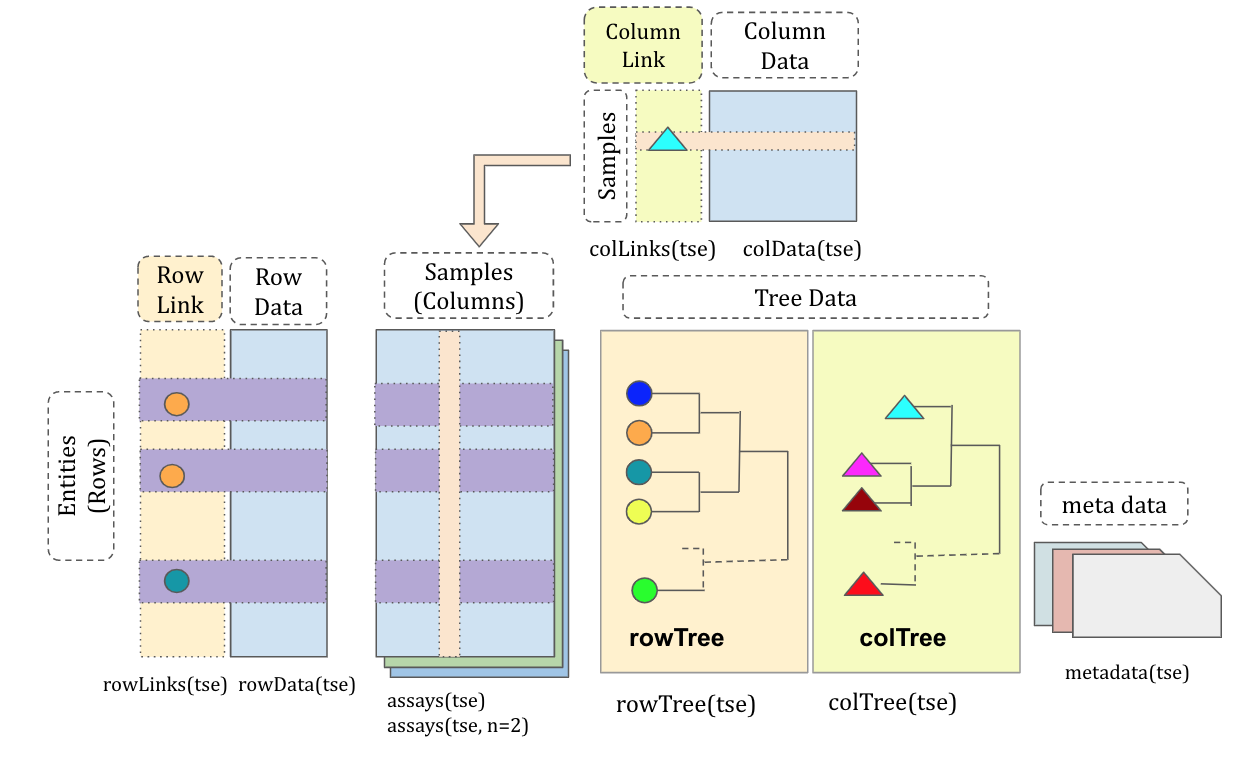
\includegraphics[width=1\linewidth,]{tse} \caption{The structure of the TreeSummarizedExperiment class.}\label{fig:use-knitr}
\end{figure}

The \texttt{rowTree} and \texttt{colTree} could be empty (\texttt{NULL}) if no trees are available.
Correspondingly, the \texttt{rowLinks} and \texttt{colLinks} would be \texttt{NULL}. All the other
slots in \texttt{TreeSummarizedExperiment} are inherited from \texttt{SingleCellExperiment} (Lun and Risso 2020).

The slots \texttt{rowTree} and \texttt{colTree} only accept the tree data as the \texttt{phylo}
class. If a tree is available in other formats, one would need to convert it to \texttt{phylo} with other R packages (e.g., \emph{\href{https://bioconductor.org/packages/3.11/treeio}{treeio}} (Wang et al. 2019)).

The \emph{\href{https://bioconductor.org/packages/3.11/TreeSummarizedExperiment}{TreeSummarizedExperiment}} package provides functions that could be separated into two main types. Functions in the first type directly work on the \texttt{TreeSummarizedExperiment} class (e.g., constructors and accessors); and others work on the tree (\texttt{phylo}) class. The latter is used mainly to create customized functions on the \texttt{TreeSummarizedExperiment} class. Also, users are freely to use functions available in other R packages to manipulate the \texttt{phylo} class (e.g., \emph{\href{https://CRAN.R-project.org/package=ape}{ape}} (Paradis and Schliep 2019)).

\hypertarget{methods}{%
\section{Methods}\label{methods}}

\hypertarget{implementation}{%
\subsection{Implementation}\label{implementation}}

\begin{Shaded}
\begin{Highlighting}[]
\KeywordTok{library}\NormalTok{(TreeSummarizedExperiment)}
\end{Highlighting}
\end{Shaded}

We generate a toy datset that has observations of 6 entities collected from 4
samples as an example to show how to construct the \texttt{TreeSummarizedExperment} object.

\begin{Shaded}
\begin{Highlighting}[]
\CommentTok{# assays data}
\NormalTok{assay_data <-}\StringTok{ }\KeywordTok{rbind}\NormalTok{(}\KeywordTok{rep}\NormalTok{(}\DecValTok{0}\NormalTok{, }\DecValTok{4}\NormalTok{), }\KeywordTok{matrix}\NormalTok{(}\DecValTok{1}\OperatorTok{:}\DecValTok{20}\NormalTok{, }\DataTypeTok{nrow =} \DecValTok{5}\NormalTok{))}
\KeywordTok{colnames}\NormalTok{(assay_data) <-}\StringTok{ }\KeywordTok{paste}\NormalTok{(}\KeywordTok{rep}\NormalTok{(LETTERS[}\DecValTok{1}\OperatorTok{:}\DecValTok{2}\NormalTok{], }\DataTypeTok{each =} \DecValTok{2}\NormalTok{), }
                            \KeywordTok{rep}\NormalTok{(}\DecValTok{1}\OperatorTok{:}\DecValTok{2}\NormalTok{, }\DecValTok{2}\NormalTok{), }\DataTypeTok{sep =} \StringTok{"_"}\NormalTok{)}
\KeywordTok{rownames}\NormalTok{(assay_data) <-}\StringTok{ }\KeywordTok{paste}\NormalTok{(}\StringTok{"entity"}\NormalTok{, }\KeywordTok{seq_len}\NormalTok{(}\DecValTok{6}\NormalTok{), }\DataTypeTok{sep =} \StringTok{""}\NormalTok{)}
\NormalTok{assay_data}
\CommentTok{##         A_1 A_2 B_1 B_2}
\CommentTok{## entity1   0   0   0   0}
\CommentTok{## entity2   1   6  11  16}
\CommentTok{## entity3   2   7  12  17}
\CommentTok{## entity4   3   8  13  18}
\CommentTok{## entity5   4   9  14  19}
\CommentTok{## entity6   5  10  15  20}
\end{Highlighting}
\end{Shaded}

The information of entities and samples are given in the \textbf{row\_data} and \textbf{col\_data}, respectively.

\begin{Shaded}
\begin{Highlighting}[]
\CommentTok{# row data}
\NormalTok{row_data <-}\StringTok{ }\KeywordTok{data.frame}\NormalTok{(}\DataTypeTok{Kindom =} \KeywordTok{rep}\NormalTok{(}\StringTok{"A"}\NormalTok{, }\DecValTok{6}\NormalTok{),}
                     \DataTypeTok{Phylum =} \KeywordTok{c}\NormalTok{(}\StringTok{"B1"}\NormalTok{, }\StringTok{"B1"}\NormalTok{, }\KeywordTok{rep}\NormalTok{(}\StringTok{"B2"}\NormalTok{, }\DecValTok{4}\NormalTok{)),}
                     \DataTypeTok{Class =} \KeywordTok{c}\NormalTok{(}\StringTok{"C1"}\NormalTok{, }\StringTok{"C1"}\NormalTok{, }\StringTok{"C2"}\NormalTok{, }\StringTok{"C2"}\NormalTok{, }\StringTok{"C3"}\NormalTok{, }\StringTok{"C3"}\NormalTok{),}
                     \DataTypeTok{OTU =} \KeywordTok{c}\NormalTok{(}\StringTok{"D1"}\NormalTok{, }\StringTok{"D2"}\NormalTok{, }\StringTok{"D3"}\NormalTok{, }\StringTok{"D4"}\NormalTok{, }\StringTok{"D5"}\NormalTok{, }\StringTok{"D6"}\NormalTok{),}
                     \DataTypeTok{row.names =} \KeywordTok{rownames}\NormalTok{(assay_data),}
                     \DataTypeTok{stringsAsFactors =} \OtherTok{FALSE}\NormalTok{)}

\NormalTok{row_data}
\CommentTok{##         Kindom Phylum Class OTU}
\CommentTok{## entity1      A     B1    C1  D1}
\CommentTok{## entity2      A     B1    C1  D2}
\CommentTok{## entity3      A     B2    C2  D3}
\CommentTok{## entity4      A     B2    C2  D4}
\CommentTok{## entity5      A     B2    C3  D5}
\CommentTok{## entity6      A     B2    C3  D6}
\CommentTok{# column data}
\NormalTok{col_data <-}\StringTok{ }\KeywordTok{data.frame}\NormalTok{(}\DataTypeTok{gg =} \KeywordTok{c}\NormalTok{(}\DecValTok{1}\NormalTok{, }\DecValTok{2}\NormalTok{, }\DecValTok{3}\NormalTok{, }\DecValTok{3}\NormalTok{),}
                    \DataTypeTok{group =} \KeywordTok{rep}\NormalTok{(LETTERS[}\DecValTok{1}\OperatorTok{:}\DecValTok{2}\NormalTok{], }\DataTypeTok{each =} \DecValTok{2}\NormalTok{), }
                    \DataTypeTok{row.names =} \KeywordTok{colnames}\NormalTok{(assay_data),}
                     \DataTypeTok{stringsAsFactors =} \OtherTok{FALSE}\NormalTok{)}
\NormalTok{col_data}
\CommentTok{##     gg group}
\CommentTok{## A_1  1     A}
\CommentTok{## A_2  2     A}
\CommentTok{## B_1  3     B}
\CommentTok{## B_2  3     B}
\end{Highlighting}
\end{Shaded}

The hierarchical structure of the 6 entities and 4 samples are denoted as
\textbf{row\_tree} and \textbf{col\_tree}, respectively. The two trees are \texttt{phylo} objects randomly created with \texttt{rtree} from the package \emph{\href{https://CRAN.R-project.org/package=ape}{ape}}.

\begin{Shaded}
\begin{Highlighting}[]
\KeywordTok{library}\NormalTok{(ape)}

\CommentTok{# The first toy tree }
\KeywordTok{set.seed}\NormalTok{(}\DecValTok{12}\NormalTok{)}
\NormalTok{row_tree <-}\StringTok{ }\KeywordTok{rtree}\NormalTok{(}\DecValTok{5}\NormalTok{)}

\CommentTok{# The second toy tree }
\KeywordTok{set.seed}\NormalTok{(}\DecValTok{12}\NormalTok{)}
\NormalTok{col_tree <-}\StringTok{ }\KeywordTok{rtree}\NormalTok{(}\DecValTok{4}\NormalTok{)}

\CommentTok{# change node labels}
\NormalTok{col_tree}\OperatorTok{$}\NormalTok{tip.label <-}\StringTok{ }\KeywordTok{colnames}\NormalTok{(assay_data)}
\NormalTok{col_tree}\OperatorTok{$}\NormalTok{node.label <-}\StringTok{ }\KeywordTok{c}\NormalTok{(}\StringTok{"All"}\NormalTok{, }\StringTok{"GroupA"}\NormalTok{, }\StringTok{"GroupB"}\NormalTok{)}
\end{Highlighting}
\end{Shaded}

We visualize the tree using the package \emph{\href{https://bioconductor.org/packages/3.11/ggtree}{ggtree}} (Yu et al. 2017). The node labels and the node numbers are in blue and orange texts, respectively. Here, the
internal nodes of the \textbf{row\_tree} have no labels.

\begin{Shaded}
\begin{Highlighting}[]
\KeywordTok{library}\NormalTok{(ggtree)}
\KeywordTok{library}\NormalTok{(ggplot2)}

\CommentTok{# Visualize the row tree}
\KeywordTok{ggtree}\NormalTok{(row_tree, }\DataTypeTok{size =} \DecValTok{2}\NormalTok{, }\DataTypeTok{branch.length =} \StringTok{"none"}\NormalTok{) }\OperatorTok{+}
\KeywordTok{geom_text2}\NormalTok{(}\KeywordTok{aes}\NormalTok{(}\DataTypeTok{label =}\NormalTok{ node), }\DataTypeTok{color =} \StringTok{"darkblue"}\NormalTok{,}
                \DataTypeTok{hjust =} \FloatTok{-0.5}\NormalTok{, }\DataTypeTok{vjust =} \FloatTok{0.7}\NormalTok{, }\DataTypeTok{size =} \DecValTok{4}\NormalTok{) }\OperatorTok{+}
\KeywordTok{geom_text2}\NormalTok{(}\KeywordTok{aes}\NormalTok{(}\DataTypeTok{label =}\NormalTok{ label), }\DataTypeTok{color =} \StringTok{"darkorange"}\NormalTok{,}
            \DataTypeTok{hjust =} \FloatTok{-0.1}\NormalTok{, }\DataTypeTok{vjust =} \FloatTok{-0.7}\NormalTok{, }\DataTypeTok{size =} \DecValTok{4}\NormalTok{) }\OperatorTok{+}
\StringTok{  }\KeywordTok{ylim}\NormalTok{(}\KeywordTok{c}\NormalTok{(}\FloatTok{0.8}\NormalTok{, }\FloatTok{5.5}\NormalTok{))}
\end{Highlighting}
\end{Shaded}

\begin{figure}
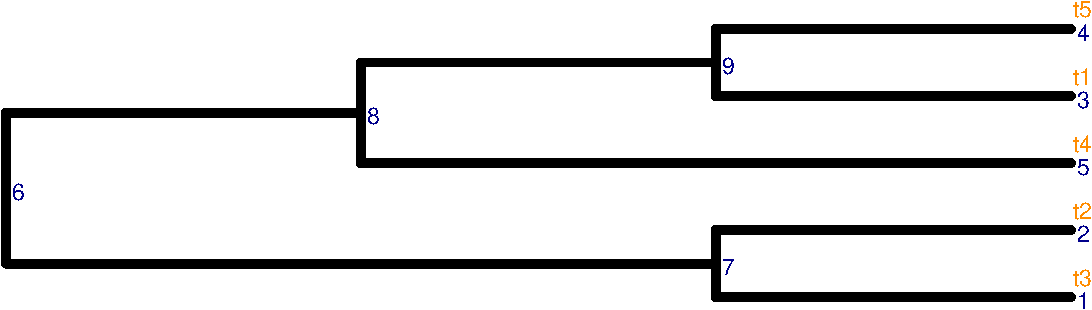
\includegraphics{figure/rtree-1} \caption{\label{rtree} The structure of the row tree}\label{fig:rtree}
\end{figure}

The \textbf{col\_tree} has labels for internal nodes.

\begin{Shaded}
\begin{Highlighting}[]
\CommentTok{# Visualize the column tree}
\KeywordTok{ggtree}\NormalTok{(col_tree, }\DataTypeTok{size =} \DecValTok{2}\NormalTok{, }\DataTypeTok{branch.length =} \StringTok{"none"}\NormalTok{) }\OperatorTok{+}
\KeywordTok{geom_text2}\NormalTok{(}\KeywordTok{aes}\NormalTok{(}\DataTypeTok{label =}\NormalTok{ node), }\DataTypeTok{color =} \StringTok{"darkblue"}\NormalTok{,}
                \DataTypeTok{hjust =} \FloatTok{-0.5}\NormalTok{, }\DataTypeTok{vjust =} \FloatTok{0.7}\NormalTok{, }\DataTypeTok{size =} \DecValTok{4}\NormalTok{) }\OperatorTok{+}
\KeywordTok{geom_text2}\NormalTok{(}\KeywordTok{aes}\NormalTok{(}\DataTypeTok{label =}\NormalTok{ label), }\DataTypeTok{color =} \StringTok{"darkorange"}\NormalTok{,}
            \DataTypeTok{hjust =} \FloatTok{-0.1}\NormalTok{, }\DataTypeTok{vjust =} \FloatTok{-0.7}\NormalTok{, }\DataTypeTok{size =} \DecValTok{4}\NormalTok{)}\OperatorTok{+}
\StringTok{  }\KeywordTok{ylim}\NormalTok{(}\KeywordTok{c}\NormalTok{(}\FloatTok{0.8}\NormalTok{, }\FloatTok{4.5}\NormalTok{)) }\OperatorTok{+}
\StringTok{  }\KeywordTok{xlim}\NormalTok{(}\KeywordTok{c}\NormalTok{(}\DecValTok{0}\NormalTok{, }\FloatTok{2.2}\NormalTok{))}
\end{Highlighting}
\end{Shaded}

\begin{figure}
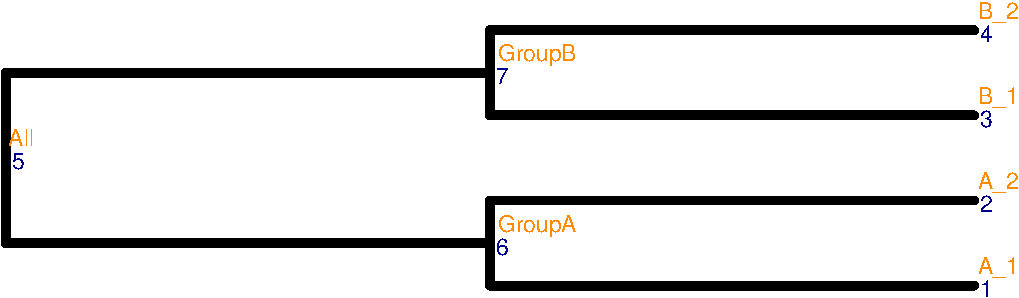
\includegraphics{figure/ctree-1} \caption{\label{ctree} The structure of the column tree}\label{fig:ctree}
\end{figure}

\hypertarget{the-construction-of-treesummarizedexperiment}{%
\subsubsection{\texorpdfstring{The construction of \texttt{TreeSummarizedExperiment}}{The construction of TreeSummarizedExperiment}}\label{the-construction-of-treesummarizedexperiment}}

The \texttt{TreeSummarizedExperiment} class is used to store the toy data:
\textbf{assay\_data}, \textbf{row\_data}, \textbf{col\_data}, \textbf{col\_tree} and \textbf{row\_tree}, To
correctly store data, the link information between the rows (or columns) of
\textbf{assay\_data} and the nodes of the \textbf{row\_tree} (or \textbf{col\_tree}) is required
to provide via a character vector \texttt{rowNodeLab} (or \texttt{colNodeLab}). Those columns
or rows that mismatch with nodes of the tree are removed with
warnings. The link data between the \texttt{assays} tables and the tree data is
automatically generated in the construction.

The row and the column trees are allowed to be included simultaneously in the
construction. As the column names of the \texttt{assays} table and the node labels of the column tree are consistent, we omit the step of providing \texttt{colNodeLab}.

\begin{Shaded}
\begin{Highlighting}[]
\CommentTok{# provide the node labels in rowNodeLab}
\NormalTok{tip_lab <-}\StringTok{ }\NormalTok{row_tree}\OperatorTok{$}\NormalTok{tip.label}
\NormalTok{row_lab <-}\StringTok{ }\NormalTok{tip_lab[}\KeywordTok{c}\NormalTok{(}\DecValTok{1}\NormalTok{, }\DecValTok{1}\OperatorTok{:}\DecValTok{5}\NormalTok{)]}
\KeywordTok{all}\NormalTok{(}\KeywordTok{colnames}\NormalTok{(assay_data) }\OperatorTok\StringTok{ }\KeywordTok{c}\NormalTok{(col_tree}\OperatorTok{$}\NormalTok{tip.label, col_tree}\OperatorTok{$}\NormalTok{node.label))}
\CommentTok{## [1] TRUE}

\NormalTok{both_tse <-}\StringTok{ }\KeywordTok{TreeSummarizedExperiment}\NormalTok{(}\DataTypeTok{assays =} \KeywordTok{list}\NormalTok{(assay_data),}
                                \DataTypeTok{rowData =}\NormalTok{ row_data,}
                                \DataTypeTok{colData =}\NormalTok{ col_data,}
                                \DataTypeTok{rowTree =}\NormalTok{ row_tree,}
                                \DataTypeTok{rowNodeLab =}\NormalTok{ row_lab,}
                                \DataTypeTok{colTree =}\NormalTok{ col_tree)}
\end{Highlighting}
\end{Shaded}

\begin{Shaded}
\begin{Highlighting}[]
\NormalTok{both_tse}
\CommentTok{## class: TreeSummarizedExperiment }
\CommentTok{## dim: 6 4 }
\CommentTok{## metadata(0):}
\CommentTok{## assays(1): ''}
\CommentTok{## rownames(6): entity1 entity2 ... entity5 entity6}
\CommentTok{## rowData names(4): Kindom Phylum Class OTU}
\CommentTok{## colnames(4): A_1 A_2 B_1 B_2}
\CommentTok{## colData names(2): gg group}
\CommentTok{## reducedDimNames(0):}
\CommentTok{## altExpNames(0):}
\CommentTok{## rowLinks: a LinkDataFrame (6 rows)}
\CommentTok{## rowTree: a phylo (5 leaves)}
\CommentTok{## colLinks: a LinkDataFrame (4 rows)}
\CommentTok{## colTree: a phylo (4 leaves)}
\end{Highlighting}
\end{Shaded}

When printing out \textbf{both\_tse}, we see a similar message as
\texttt{SingleCellExperiment} (Lun and Risso 2020) with four additional lines about \texttt{rowLinks}, \texttt{rowTree},
\texttt{colLinks} and \texttt{colTree}.

\hypertarget{the-accessor-functions}{%
\subsubsection{The accessor functions}\label{the-accessor-functions}}

For slots inherited from the family of \texttt{SummarizedExperiment} class, they could be accessed in the traditional way.

\begin{Shaded}
\begin{Highlighting}[]
\CommentTok{# access assays}
\KeywordTok{assays}\NormalTok{(both_tse)}

\CommentTok{# the row data}
\KeywordTok{rowData}\NormalTok{(both_tse)}

\CommentTok{# the column data}
\KeywordTok{colData}\NormalTok{(both_tse)}

\CommentTok{# the metadata: it's empty here}
\KeywordTok{metadata}\NormalTok{(both_tse)}
\end{Highlighting}
\end{Shaded}

For new slots, we provide \texttt{rowTree} (\texttt{colTree}) to access the row (column) trees, and \texttt{rowLinks} (\texttt{colLinks}) to access the link information between \texttt{assays} and nodes of the row (column) tree. If the tree is not available, the corresponding link data is \texttt{NULL}.

\begin{Shaded}
\begin{Highlighting}[]
\CommentTok{# access trees}
\KeywordTok{rowTree}\NormalTok{(both_tse)}
\CommentTok{## }
\CommentTok{## Phylogenetic tree with 5 tips and 4 internal nodes.}
\CommentTok{## }
\CommentTok{## Tip labels:}
\CommentTok{## [1] "t3" "t2" "t1" "t5" "t4"}
\CommentTok{## }
\CommentTok{## Rooted; includes branch lengths.}
\KeywordTok{colTree}\NormalTok{(both_tse)}
\CommentTok{## }
\CommentTok{## Phylogenetic tree with 4 tips and 3 internal nodes.}
\CommentTok{## }
\CommentTok{## Tip labels:}
\CommentTok{## [1] "A_1" "A_2" "B_1" "B_2"}
\CommentTok{## Node labels:}
\CommentTok{## [1] "All"    "GroupA" "GroupB"}
\CommentTok{## }
\CommentTok{## Rooted; includes branch lengths.}
\end{Highlighting}
\end{Shaded}

\begin{Shaded}
\begin{Highlighting}[]
\CommentTok{# access the link data}
\NormalTok{(rLink <-}\StringTok{ }\KeywordTok{rowLinks}\NormalTok{(both_tse))}
\CommentTok{## LinkDataFrame with 6 rows and 4 columns}
\CommentTok{##             nodeLab nodeLab_alias   nodeNum    isLeaf}
\CommentTok{##         <character>   <character> <integer> <logical>}
\CommentTok{## entity1          t3       alias_1         1      TRUE}
\CommentTok{## entity2          t3       alias_1         1      TRUE}
\CommentTok{## entity3          t2       alias_2         2      TRUE}
\CommentTok{## entity4          t1       alias_3         3      TRUE}
\CommentTok{## entity5          t5       alias_4         4      TRUE}
\CommentTok{## entity6          t4       alias_5         5      TRUE}
\NormalTok{(cLink <-}\StringTok{ }\KeywordTok{colLinks}\NormalTok{(both_tse))}
\CommentTok{## LinkDataFrame with 4 rows and 4 columns}
\CommentTok{##         nodeLab nodeLab_alias   nodeNum    isLeaf}
\CommentTok{##     <character>   <character> <integer> <logical>}
\CommentTok{## A_1         A_1       alias_1         1      TRUE}
\CommentTok{## A_2         A_2       alias_2         2      TRUE}
\CommentTok{## B_1         B_1       alias_3         3      TRUE}
\CommentTok{## B_2         B_2       alias_4         4      TRUE}
\end{Highlighting}
\end{Shaded}

The link data has the \texttt{LinkDataFrame} class that is extended from the \texttt{DataFrame} class with the restriction that it has at least four columns:
\textbf{nodeLab}, \textbf{nodeLab\_alias}, \textbf{nodeNum}, and \textbf{isLeaf}. More details about
the \texttt{DataFrame} class could be found in the \emph{\href{https://bioconductor.org/packages/3.11/S4Vectors}{S4Vectors}} package.

\begin{itemize}
\tightlist
\item
  nodeLab: the labels of nodes on the tree
\item
  nodeLab\_alias: the alias labels of nodes on the tree
\item
  nodeNum: the numbers of nodes on the tree
\item
  isLeaf: whether the node is a leaf node
\end{itemize}

\hypertarget{the-subseting-function}{%
\subsubsection{The subseting function}\label{the-subseting-function}}

Two ways are available to subset a \texttt{TreeSummarizedExperiment} object: \texttt{{[}} to
subset by rows or columns, and \texttt{subsetByNode} to subset by nodes of a tree. To
keep track of the original data, the \texttt{rowTree} and \texttt{colTree} stay the same after
subseting.

\begin{Shaded}
\begin{Highlighting}[]
\NormalTok{sub_tse <-}\StringTok{ }\NormalTok{both_tse[}\DecValTok{1}\OperatorTok{:}\DecValTok{2}\NormalTok{, }\DecValTok{1}\NormalTok{]}
\NormalTok{sub_tse}
\CommentTok{## class: TreeSummarizedExperiment }
\CommentTok{## dim: 2 1 }
\CommentTok{## metadata(0):}
\CommentTok{## assays(1): ''}
\CommentTok{## rownames(2): entity1 entity2}
\CommentTok{## rowData names(4): Kindom Phylum Class OTU}
\CommentTok{## colnames(1): A_1}
\CommentTok{## colData names(2): gg group}
\CommentTok{## reducedDimNames(0):}
\CommentTok{## altExpNames(0):}
\CommentTok{## rowLinks: a LinkDataFrame (2 rows)}
\CommentTok{## rowTree: a phylo (5 leaves)}
\CommentTok{## colLinks: a LinkDataFrame (1 rows)}
\CommentTok{## colTree: a phylo (4 leaves)}
\end{Highlighting}
\end{Shaded}

\texttt{rowLinks} and \texttt{rowData} are updated accordingly.

\begin{Shaded}
\begin{Highlighting}[]
\CommentTok{# The first four columns are from rowLinks data and the others from the rowData}
\KeywordTok{cbind}\NormalTok{(}\KeywordTok{rowLinks}\NormalTok{(sub_tse), }\KeywordTok{rowData}\NormalTok{(sub_tse))}
\CommentTok{## DataFrame with 2 rows and 8 columns}
\CommentTok{##             nodeLab nodeLab_alias   nodeNum    isLeaf      Kindom      Phylum}
\CommentTok{##         <character>   <character> <integer> <logical> <character> <character>}
\CommentTok{## entity1          t3       alias_1         1      TRUE           A          B1}
\CommentTok{## entity2          t3       alias_1         1      TRUE           A          B1}
\CommentTok{##               Class         OTU}
\CommentTok{##         <character> <character>}
\CommentTok{## entity1          C1          D1}
\CommentTok{## entity2          C1          D2}
\end{Highlighting}
\end{Shaded}

\begin{Shaded}
\begin{Highlighting}[]
\CommentTok{# The first four columns are from colLinks data and the others from colData}
\KeywordTok{cbind}\NormalTok{(}\KeywordTok{colLinks}\NormalTok{(sub_tse), }\KeywordTok{colData}\NormalTok{(sub_tse))}
\CommentTok{## DataFrame with 1 row and 6 columns}
\CommentTok{##         nodeLab nodeLab_alias   nodeNum    isLeaf        gg       group}
\CommentTok{##     <character>   <character> <integer> <logical> <numeric> <character>}
\CommentTok{## A_1         A_1       alias_1         1      TRUE         1           A}
\end{Highlighting}
\end{Shaded}

To subset by nodes, we specify the node by its node label or node number. Here, \emph{entity1} and \emph{entity2} are both mapped to the same node \texttt{t3}, so both of them are obtained.

\begin{Shaded}
\begin{Highlighting}[]
\NormalTok{node_tse <-}\StringTok{ }\KeywordTok{subsetByNode}\NormalTok{(}\DataTypeTok{x =}\NormalTok{ both_tse, }\DataTypeTok{rowNode =} \StringTok{"t3"}\NormalTok{)}

\KeywordTok{rowLinks}\NormalTok{(node_tse)}
\CommentTok{## LinkDataFrame with 2 rows and 4 columns}
\CommentTok{##             nodeLab nodeLab_alias   nodeNum    isLeaf}
\CommentTok{##         <character>   <character> <integer> <logical>}
\CommentTok{## entity1          t3       alias_1         1      TRUE}
\CommentTok{## entity2          t3       alias_1         1      TRUE}
\end{Highlighting}
\end{Shaded}

It is allowed to subset simultaneously in both dimensions.

\begin{Shaded}
\begin{Highlighting}[]
\NormalTok{node_tse <-}\StringTok{ }\KeywordTok{subsetByNode}\NormalTok{(}\DataTypeTok{x =}\NormalTok{ both_tse, }\DataTypeTok{rowNode =} \StringTok{"t3"}\NormalTok{, }
                         \DataTypeTok{colNode =} \KeywordTok{c}\NormalTok{(}\StringTok{"A_1"}\NormalTok{, }\StringTok{"A_2"}\NormalTok{))}
\KeywordTok{assays}\NormalTok{(node_tse)[[}\DecValTok{1}\NormalTok{]]}
\CommentTok{##         A_1 A_2}
\CommentTok{## entity1   0   0}
\CommentTok{## entity2   1   6}
\end{Highlighting}
\end{Shaded}

\hypertarget{change-the-tree}{%
\subsubsection{Change the tree}\label{change-the-tree}}

The current tree is allowed to be replaced by a new one by using the \texttt{changeTree}. If the hierarchical information is available as a \texttt{data.frame} with each column representing a taxonomic level (e.g., \emph{row\_data}), we provide \texttt{toTree} to convert it into a \texttt{phylo} object.

\begin{Shaded}
\begin{Highlighting}[]
\CommentTok{# The toy taxonomic table}
\NormalTok{taxa <-}\StringTok{ }\KeywordTok{rowData}\NormalTok{(both_tse)}

\CommentTok{# convert it to a phylo tree}
\NormalTok{taxa_tree <-}\StringTok{ }\KeywordTok{toTree}\NormalTok{(}\DataTypeTok{data =}\NormalTok{ taxa)}

\CommentTok{# Viz the new tree}
\KeywordTok{ggtree}\NormalTok{(taxa_tree)}\OperatorTok{+}
\KeywordTok{geom_text2}\NormalTok{(}\KeywordTok{aes}\NormalTok{(}\DataTypeTok{label =}\NormalTok{ node), }\DataTypeTok{color =} \StringTok{"darkblue"}\NormalTok{,}
                \DataTypeTok{hjust =} \FloatTok{-0.5}\NormalTok{, }\DataTypeTok{vjust =} \FloatTok{0.7}\NormalTok{, }\DataTypeTok{size =} \DecValTok{4}\NormalTok{) }\OperatorTok{+}
\KeywordTok{geom_text2}\NormalTok{(}\KeywordTok{aes}\NormalTok{(}\DataTypeTok{label =}\NormalTok{ label), }\DataTypeTok{color =} \StringTok{"darkorange"}\NormalTok{,}
            \DataTypeTok{hjust =} \FloatTok{-0.1}\NormalTok{, }\DataTypeTok{vjust =} \FloatTok{-0.7}\NormalTok{, }\DataTypeTok{size =} \DecValTok{4}\NormalTok{) }\OperatorTok{+}
\StringTok{    }\KeywordTok{geom_point2}\NormalTok{()}
\end{Highlighting}
\end{Shaded}

\begin{adjustwidth}{\fltoffset}{0mm}
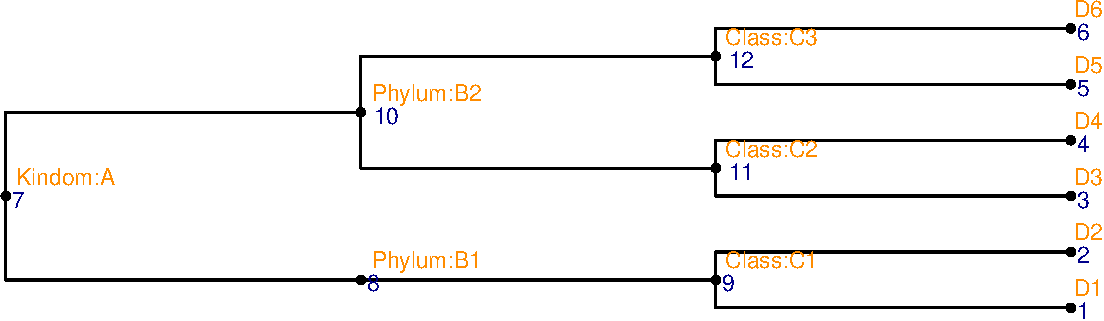
\includegraphics{figure/unnamed-chunk-15-1} \end{adjustwidth}

The information to match nodes of two trees are required if nodes are labeled differently.

\begin{Shaded}
\begin{Highlighting}[]
\NormalTok{taxa_tse <-}\StringTok{ }\KeywordTok{changeTree}\NormalTok{(}\DataTypeTok{x =}\NormalTok{ both_tse, }\DataTypeTok{rowTree =}\NormalTok{ taxa_tree, }
                       \DataTypeTok{rowNodeLab =}\NormalTok{ taxa[[}\StringTok{"OTU"}\NormalTok{]])}

\NormalTok{taxa_tse}
\CommentTok{## class: TreeSummarizedExperiment }
\CommentTok{## dim: 6 4 }
\CommentTok{## metadata(0):}
\CommentTok{## assays(1): ''}
\CommentTok{## rownames(6): entity1 entity2 ... entity5 entity6}
\CommentTok{## rowData names(4): Kindom Phylum Class OTU}
\CommentTok{## colnames(4): A_1 A_2 B_1 B_2}
\CommentTok{## colData names(2): gg group}
\CommentTok{## reducedDimNames(0):}
\CommentTok{## altExpNames(0):}
\CommentTok{## rowLinks: a LinkDataFrame (6 rows)}
\CommentTok{## rowTree: a phylo (6 leaves)}
\CommentTok{## colLinks: a LinkDataFrame (4 rows)}
\CommentTok{## colTree: a phylo (4 leaves)}
\KeywordTok{rowLinks}\NormalTok{(taxa_tse)}
\CommentTok{## LinkDataFrame with 6 rows and 4 columns}
\CommentTok{##             nodeLab nodeLab_alias   nodeNum    isLeaf}
\CommentTok{##         <character>   <character> <integer> <logical>}
\CommentTok{## entity1          D1       alias_1         1      TRUE}
\CommentTok{## entity2          D2       alias_2         2      TRUE}
\CommentTok{## entity3          D3       alias_3         3      TRUE}
\CommentTok{## entity4          D4       alias_4         4      TRUE}
\CommentTok{## entity5          D5       alias_5         5      TRUE}
\CommentTok{## entity6          D6       alias_6         6      TRUE}
\end{Highlighting}
\end{Shaded}

\hypertarget{aggregation}{%
\subsubsection{Aggregation}\label{aggregation}}

Data can be flexibly aggregated to different levels of the tree.

\hypertarget{aggCol}{%
\paragraph{The column dimension}\label{aggCol}}

Here, we show the aggregation on the column dimension. The
\texttt{TreeSummarizedExperiment} object is assigned to the argument \texttt{x}. The desired
aggregation level is given in \texttt{colLevel}. The level could be specified via the
node label (the orange texts in Figure \ref{fig:ctree}) or the node number (the
blue texts in Figure \ref{fig:ctree}). We could further decide how to aggregate
via the argument \texttt{FUN}.

\begin{Shaded}
\begin{Highlighting}[]
\CommentTok{# use node labels to specify colLevel}
\NormalTok{aggCol <-}\StringTok{ }\KeywordTok{aggValue}\NormalTok{(}\DataTypeTok{x =}\NormalTok{ taxa_tse, }
                   \DataTypeTok{colLevel =} \KeywordTok{c}\NormalTok{(}\StringTok{"GroupA"}\NormalTok{, }\StringTok{"GroupB"}\NormalTok{),}
                   \DataTypeTok{FUN =}\NormalTok{ sum)}
\CommentTok{# or use node numbers to specify colLevel}
\NormalTok{aggCol <-}\StringTok{ }\KeywordTok{aggValue}\NormalTok{(}\DataTypeTok{x =}\NormalTok{ taxa_tse, }\DataTypeTok{colLevel =} \KeywordTok{c}\NormalTok{(}\DecValTok{6}\NormalTok{, }\DecValTok{7}\NormalTok{), }\DataTypeTok{FUN =}\NormalTok{ sum)}
\end{Highlighting}
\end{Shaded}

\begin{Shaded}
\begin{Highlighting}[]
\KeywordTok{assays}\NormalTok{(aggCol)[[}\DecValTok{1}\NormalTok{]]}
\CommentTok{##         alias_6 alias_7}
\CommentTok{## entity1       0       0}
\CommentTok{## entity2       7      27}
\CommentTok{## entity3       9      29}
\CommentTok{## entity4      11      31}
\CommentTok{## entity5      13      33}
\CommentTok{## entity6      15      35}
\end{Highlighting}
\end{Shaded}

The \texttt{rowData} does not change, but the \texttt{colData} adjusts with the change of the
\texttt{assays} table. For example, the column \textbf{group} has the \texttt{A} value for
\texttt{GroupA} because the descendant nodes of \texttt{GroupA} all have the value \texttt{A}; the
column \textbf{gg} has the \texttt{NA} value for \texttt{GroupA} because the descendant nodes of
\texttt{GroupA} have different values, (1 and 2).

\begin{Shaded}
\begin{Highlighting}[]
\CommentTok{# before aggregation}
\KeywordTok{colData}\NormalTok{(taxa_tse)}
\CommentTok{## DataFrame with 4 rows and 2 columns}
\CommentTok{##            gg       group}
\CommentTok{##     <numeric> <character>}
\CommentTok{## A_1         1           A}
\CommentTok{## A_2         2           A}
\CommentTok{## B_1         3           B}
\CommentTok{## B_2         3           B}
\CommentTok{# after aggregation}
\KeywordTok{colData}\NormalTok{(aggCol)}
\CommentTok{## DataFrame with 2 rows and 2 columns}
\CommentTok{##                gg       group}
\CommentTok{##         <numeric> <character>}
\CommentTok{## alias_6        NA           A}
\CommentTok{## alias_7         3           B}
\end{Highlighting}
\end{Shaded}

The \texttt{colLinks} is updated to link the new rows of \texttt{assays} tables and the column
tree.

\begin{Shaded}
\begin{Highlighting}[]
\CommentTok{# the link data is updated}
\KeywordTok{colLinks}\NormalTok{(aggCol)}
\CommentTok{## LinkDataFrame with 2 rows and 4 columns}
\CommentTok{##             nodeLab nodeLab_alias   nodeNum    isLeaf}
\CommentTok{##         <character>   <character> <integer> <logical>}
\CommentTok{## alias_6      GroupA       alias_6         6     FALSE}
\CommentTok{## alias_7      GroupB       alias_7         7     FALSE}
\end{Highlighting}
\end{Shaded}

From the Figure \ref{fig:rtree}, we could see that the nodes 6 and 7 are
labeled with \texttt{GroupA} and \texttt{GroupB}, respectively. This agrees with the
column link data.

\hypertarget{aggRow}{%
\paragraph{The row dimension}\label{aggRow}}

Similarly, we could aggregate the data to the phylum level by providing the internal nodes that represent the phylum level, \texttt{taxa\_one}.

\begin{Shaded}
\begin{Highlighting}[]
\CommentTok{# the phylum level}
\NormalTok{taxa <-}\StringTok{ }\KeywordTok{c}\NormalTok{(taxa_tree}\OperatorTok{$}\NormalTok{tip.label, taxa_tree}\OperatorTok{$}\NormalTok{node.label)}
\NormalTok{(taxa_one <-}\StringTok{ }\NormalTok{taxa[}\KeywordTok{startsWith}\NormalTok{(taxa, }\StringTok{"Phylum:"}\NormalTok{)])}
\CommentTok{## [1] "Phylum:B1" "Phylum:B2"}

\CommentTok{# aggregation}
\NormalTok{agg_taxa <-}\StringTok{ }\KeywordTok{aggValue}\NormalTok{(}\DataTypeTok{x =}\NormalTok{ taxa_tse, }\DataTypeTok{rowLevel =}\NormalTok{ taxa_one, }\DataTypeTok{FUN =}\NormalTok{ sum)}
\NormalTok{agg_taxa}
\CommentTok{## class: TreeSummarizedExperiment }
\CommentTok{## dim: 2 4 }
\CommentTok{## metadata(0):}
\CommentTok{## assays(1): ''}
\CommentTok{## rownames(2): alias_8 alias_10}
\CommentTok{## rowData names(4): Kindom Phylum Class OTU}
\CommentTok{## colnames(4): A_1 A_2 B_1 B_2}
\CommentTok{## colData names(2): gg group}
\CommentTok{## reducedDimNames(0):}
\CommentTok{## altExpNames(0):}
\CommentTok{## rowLinks: a LinkDataFrame (2 rows)}
\CommentTok{## rowTree: a phylo (6 leaves)}
\CommentTok{## colLinks: a LinkDataFrame (4 rows)}
\CommentTok{## colTree: a phylo (4 leaves)}
\end{Highlighting}
\end{Shaded}

It's free to choose nodes from different taxonomic ranks.

\begin{Shaded}
\begin{Highlighting}[]
\CommentTok{# A mixed level}
\NormalTok{taxa_mix <-}\StringTok{ }\KeywordTok{c}\NormalTok{(}\StringTok{"Class:C3"}\NormalTok{, }\StringTok{"Phylum:B1"}\NormalTok{)}
\NormalTok{agg_any <-}\StringTok{ }\KeywordTok{aggValue}\NormalTok{(}\DataTypeTok{x =}\NormalTok{ taxa_tse, }\DataTypeTok{rowLevel =}\NormalTok{ taxa_mix, }\DataTypeTok{FUN =}\NormalTok{ sum)}
\KeywordTok{rowData}\NormalTok{(agg_any)}
\CommentTok{## DataFrame with 2 rows and 4 columns}
\CommentTok{##               Kindom      Phylum       Class       OTU}
\CommentTok{##          <character> <character> <character> <logical>}
\CommentTok{## alias_12           A          B2          C3        NA}
\CommentTok{## alias_8            A          B1          C1        NA}
\end{Highlighting}
\end{Shaded}

\hypertarget{both-dimensions}{%
\paragraph{Both dimensions}\label{both-dimensions}}

The aggregation on both dimensions could be performed in one step using the same
function specified via \texttt{FUN}. If different functions are required for different
dimensions, the aggregation should be performed in two steps because the aggregation order matters.

\begin{Shaded}
\begin{Highlighting}[]
\NormalTok{agg_both <-}\StringTok{ }\KeywordTok{aggValue}\NormalTok{(}\DataTypeTok{x =}\NormalTok{ both_tse, }\DataTypeTok{colLevel =} \KeywordTok{c}\NormalTok{(}\DecValTok{6}\NormalTok{, }\DecValTok{7}\NormalTok{), }
                    \DataTypeTok{rowLevel =} \DecValTok{7}\OperatorTok{:}\DecValTok{9}\NormalTok{, }\DataTypeTok{FUN =}\NormalTok{ sum)}
\end{Highlighting}
\end{Shaded}

As expected, we obtain a table with 3 rows (\texttt{rowLevel = 7:9}) and 2 columns
(\texttt{colLevel = c(6, 7)}).

\begin{Shaded}
\begin{Highlighting}[]
\KeywordTok{assays}\NormalTok{(agg_both)[[}\DecValTok{1}\NormalTok{]]}
\CommentTok{##         alias_6 alias_7}
\CommentTok{## alias_7      16      56}
\CommentTok{## alias_8      39      99}
\CommentTok{## alias_9      24      64}
\end{Highlighting}
\end{Shaded}

\hypertarget{functions-working-on-the-phylo-object.}{%
\subsubsection{\texorpdfstring{Functions working on the \texttt{phylo} object.}{Functions working on the phylo object.}}\label{functions-working-on-the-phylo-object.}}

We create some functions to manipulate or to extract information
from the \texttt{phylo} object. More functions could be found in other packages, such
as \emph{\href{https://CRAN.R-project.org/package=ape}{ape}} ({\textbf{???}}), \emph{\href{https://CRAN.R-project.org/package=tidytree}{tidytree}}. These functions are
useful when users want to customize functions for the \texttt{TreeSummarizedExperiment}
class.

To show these functions, we use an example tree that has its node labels (black texts) and node numbers (blue texts) shown as below.

\begin{Shaded}
\begin{Highlighting}[]
\KeywordTok{ggtree}\NormalTok{(tinyTree, }\DataTypeTok{branch.length =} \StringTok{"none"}\NormalTok{) }\OperatorTok{+}
\StringTok{    }\KeywordTok{geom_text2}\NormalTok{(}\KeywordTok{aes}\NormalTok{(}\DataTypeTok{label =}\NormalTok{ label), }\DataTypeTok{hjust =} \FloatTok{-0.1}\NormalTok{, }\DataTypeTok{size =} \DecValTok{3}\NormalTok{) }\OperatorTok{+}
\StringTok{    }\KeywordTok{geom_text2}\NormalTok{(}\KeywordTok{aes}\NormalTok{(}\DataTypeTok{label =}\NormalTok{ node), }\DataTypeTok{vjust =} \FloatTok{-0.8}\NormalTok{,}
               \DataTypeTok{hjust =} \FloatTok{-0.2}\NormalTok{, }\DataTypeTok{color =} \StringTok{'blue'}\NormalTok{, }\DataTypeTok{size =} \DecValTok{3}\NormalTok{) }
\end{Highlighting}
\end{Shaded}

\begin{adjustwidth}{\fltoffset}{0mm}
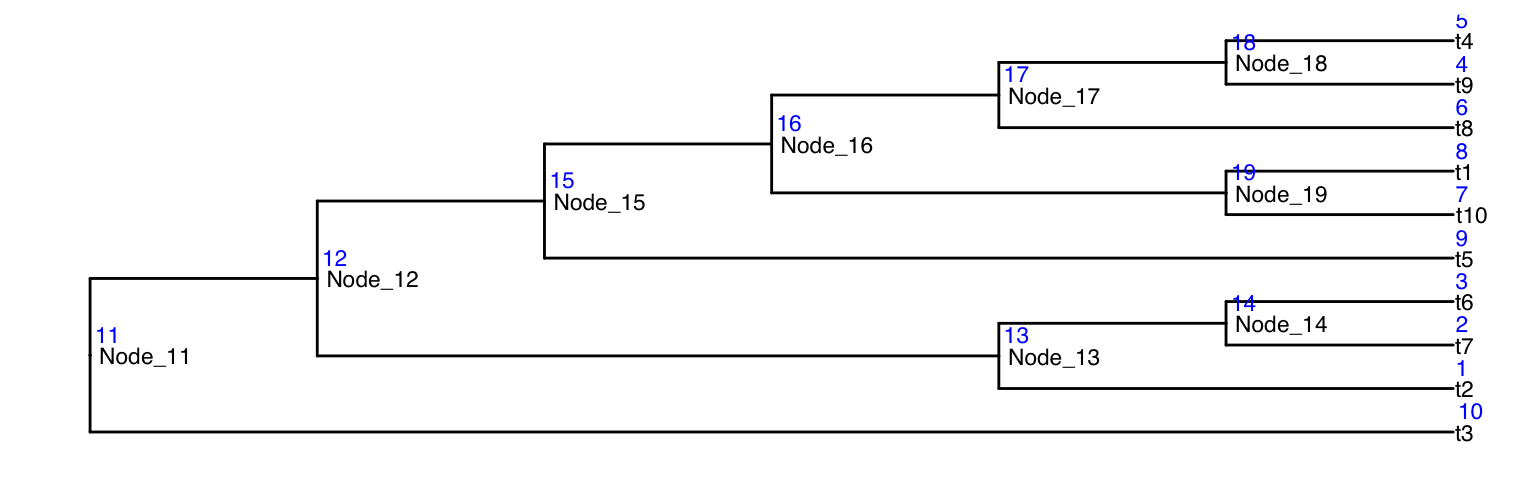
\includegraphics{figure/unnamed-chunk-25-1} \end{adjustwidth}

\hypertarget{print-out-nodes-of-the-tree}{%
\paragraph{print out nodes of the tree}\label{print-out-nodes-of-the-tree}}

We could print out all nodes (\texttt{type = "all"}), the leaves (\texttt{type = "leaf"}) or the internal nodes (\texttt{type = "internal"}) with \texttt{printNode}.

\begin{Shaded}
\begin{Highlighting}[]
\KeywordTok{printNode}\NormalTok{(}\DataTypeTok{tree =}\NormalTok{ tinyTree, }\DataTypeTok{type =} \StringTok{"all"}\NormalTok{)}
\CommentTok{##    nodeLab nodeLab_alias nodeNum isLeaf}
\CommentTok{## 1       t2        alias1       1   TRUE}
\CommentTok{## 2       t7        alias2       2   TRUE}
\CommentTok{## 3       t6        alias3       3   TRUE}
\CommentTok{## 4       t9        alias4       4   TRUE}
\CommentTok{## 5       t4        alias5       5   TRUE}
\CommentTok{## 6       t8        alias6       6   TRUE}
\CommentTok{## 7      t10        alias7       7   TRUE}
\CommentTok{## 8       t1        alias8       8   TRUE}
\CommentTok{## 9       t5        alias9       9   TRUE}
\CommentTok{## 10      t3       alias10      10   TRUE}
\CommentTok{## 11 Node_11      alias_11      11  FALSE}
\CommentTok{## 12 Node_12      alias_12      12  FALSE}
\CommentTok{## 13 Node_13      alias_13      13  FALSE}
\CommentTok{## 14 Node_14      alias_14      14  FALSE}
\CommentTok{## 15 Node_15      alias_15      15  FALSE}
\CommentTok{## 16 Node_16      alias_16      16  FALSE}
\CommentTok{## 17 Node_17      alias_17      17  FALSE}
\CommentTok{## 18 Node_18      alias_18      18  FALSE}
\CommentTok{## 19 Node_19      alias_19      19  FALSE}
\end{Highlighting}
\end{Shaded}

\hypertarget{count-the-number-of-nodes}{%
\paragraph{Count the number of nodes}\label{count-the-number-of-nodes}}

\begin{Shaded}
\begin{Highlighting}[]
\CommentTok{# The number of leaves}
\KeywordTok{countLeaf}\NormalTok{(}\DataTypeTok{tree =}\NormalTok{ tinyTree)}
\CommentTok{## [1] 10}

\CommentTok{# The number of nodes (leaf nodes and internal nodes)}
\KeywordTok{countNode}\NormalTok{(}\DataTypeTok{tree =}\NormalTok{ tinyTree)}
\CommentTok{## [1] 19}
\end{Highlighting}
\end{Shaded}

\hypertarget{conversion-of-the-node-label-and-the-node-number}{%
\paragraph{Conversion of the node label and the node number}\label{conversion-of-the-node-label-and-the-node-number}}

The translation between the labels and the numbers of nodes could be achieved by
the function \texttt{transNode}.

\begin{Shaded}
\begin{Highlighting}[]
\KeywordTok{transNode}\NormalTok{(}\DataTypeTok{tree =}\NormalTok{ tinyTree, }\DataTypeTok{node =} \KeywordTok{c}\NormalTok{(}\DecValTok{12}\NormalTok{, }\DecValTok{1}\NormalTok{, }\DecValTok{4}\NormalTok{))}
\CommentTok{## [1] "Node_12" "t2"      "t9"}
\end{Highlighting}
\end{Shaded}

\begin{Shaded}
\begin{Highlighting}[]
\KeywordTok{transNode}\NormalTok{(}\DataTypeTok{tree =}\NormalTok{ tinyTree, }\DataTypeTok{node =} \KeywordTok{c}\NormalTok{(}\StringTok{"t4"}\NormalTok{, }\StringTok{"Node_18"}\NormalTok{))}
\CommentTok{##      t4 Node_18 }
\CommentTok{##       5      18}
\end{Highlighting}
\end{Shaded}

\hypertarget{find-the-descendants}{%
\paragraph{Find the descendants}\label{find-the-descendants}}

To get descendants that are at the leaf level, we could set the argument
\texttt{only.leaf = TRUE}.

\begin{Shaded}
\begin{Highlighting}[]
\CommentTok{# only the leaf nodes}
\KeywordTok{findOS}\NormalTok{(}\DataTypeTok{tree =}\NormalTok{ tinyTree, }\DataTypeTok{node =} \DecValTok{17}\NormalTok{, }\DataTypeTok{only.leaf =} \OtherTok{TRUE}\NormalTok{)}
\CommentTok{## $Node_17}
\CommentTok{## [1] 4 5 6}
\end{Highlighting}
\end{Shaded}

The argument \texttt{only.leaf = FALSE} is set to get all descendants

\begin{Shaded}
\begin{Highlighting}[]
\CommentTok{# all descendant nodes}
\KeywordTok{findOS}\NormalTok{(}\DataTypeTok{tree =}\NormalTok{ tinyTree, }\DataTypeTok{node =} \DecValTok{17}\NormalTok{, }\DataTypeTok{only.leaf =} \OtherTok{FALSE}\NormalTok{)}
\CommentTok{## $Node_17}
\CommentTok{## [1]  4  5  6 18}
\end{Highlighting}
\end{Shaded}

\hypertarget{find-the-sibling-node}{%
\paragraph{Find the sibling node}\label{find-the-sibling-node}}

The input \texttt{node} could be either the node label or the node number.

\begin{Shaded}
\begin{Highlighting}[]
\CommentTok{# node = 5, node = "t4" are the same node}
\KeywordTok{findSibling}\NormalTok{(}\DataTypeTok{tree =}\NormalTok{ tinyTree, }\DataTypeTok{node =} \DecValTok{5}\NormalTok{)}
\CommentTok{## t9 }
\CommentTok{##  4}
\KeywordTok{findSibling}\NormalTok{(}\DataTypeTok{tree =}\NormalTok{ tinyTree, }\DataTypeTok{node =} \StringTok{"t4"}\NormalTok{)}
\CommentTok{## t9 }
\CommentTok{##  4}
\end{Highlighting}
\end{Shaded}

\hypertarget{find-the-share-node}{%
\paragraph{Find the share node}\label{find-the-share-node}}

This would find the first node that joined by the specified nodes (\texttt{node}) in
their paths to the root.

\begin{Shaded}
\begin{Highlighting}[]
\KeywordTok{shareNode}\NormalTok{(}\DataTypeTok{tree =}\NormalTok{ tinyTree, }\DataTypeTok{node =} \KeywordTok{c}\NormalTok{(}\DecValTok{5}\NormalTok{, }\DecValTok{6}\NormalTok{))}
\CommentTok{## Node_17 }
\CommentTok{##      17}
\end{Highlighting}
\end{Shaded}

\hypertarget{identify-leaf-nodes}{%
\paragraph{Identify leaf nodes}\label{identify-leaf-nodes}}

\begin{Shaded}
\begin{Highlighting}[]
\KeywordTok{isLeaf}\NormalTok{(}\DataTypeTok{tree =}\NormalTok{ tinyTree, }\DataTypeTok{node =} \DecValTok{5}\NormalTok{)}
\CommentTok{## [1] TRUE}
\KeywordTok{isLeaf}\NormalTok{(}\DataTypeTok{tree =}\NormalTok{ tinyTree, }\DataTypeTok{node =} \DecValTok{17}\NormalTok{)}
\CommentTok{## [1] FALSE}
\end{Highlighting}
\end{Shaded}

\hypertarget{the-distance-between-two-nodes}{%
\paragraph{The distance between two nodes}\label{the-distance-between-two-nodes}}

The distance between two nodes is obtained using \texttt{distNode}.

\begin{Shaded}
\begin{Highlighting}[]
\KeywordTok{distNode}\NormalTok{(}\DataTypeTok{tree =}\NormalTok{ tinyTree, }\DataTypeTok{node =} \KeywordTok{c}\NormalTok{(}\DecValTok{1}\NormalTok{, }\DecValTok{5}\NormalTok{))}
\CommentTok{## [1] 2.699212}
\end{Highlighting}
\end{Shaded}

\hypertarget{convert-a-phylo-object-to-a-matrix}{%
\paragraph{\texorpdfstring{Convert a \texttt{phylo} object to a matrix}{Convert a phylo object to a matrix}}\label{convert-a-phylo-object-to-a-matrix}}

Each row gives a path that connects a leaf and the root. Each entry value is a node reprsented by its node number.

\begin{Shaded}
\begin{Highlighting}[]
\KeywordTok{matTree}\NormalTok{(}\DataTypeTok{tree =}\NormalTok{ tinyTree)}
\CommentTok{##       L1 L2 L3 L4 L5 L6 L7}
\CommentTok{##  [1,]  1 13 12 11 NA NA NA}
\CommentTok{##  [2,]  2 14 13 12 11 NA NA}
\CommentTok{##  [3,]  3 14 13 12 11 NA NA}
\CommentTok{##  [4,]  4 18 17 16 15 12 11}
\CommentTok{##  [5,]  5 18 17 16 15 12 11}
\CommentTok{##  [6,]  6 17 16 15 12 11 NA}
\CommentTok{##  [7,]  7 19 16 15 12 11 NA}
\CommentTok{##  [8,]  8 19 16 15 12 11 NA}
\CommentTok{##  [9,]  9 15 12 11 NA NA NA}
\CommentTok{## [10,] 10 11 NA NA NA NA NA}
\end{Highlighting}
\end{Shaded}

\hypertarget{modifyLink}{%
\subsubsection{\texorpdfstring{Customize functions for the \texttt{TreeSummarizedExperiment} class}{Customize functions for the TreeSummarizedExperiment class}}\label{modifyLink}}

We show examples about how to create functions for the
\texttt{TreeSummarizedExperiment}. Here, the function \texttt{rmRows} is to remove
entities (on rows) that have zero in all samples (on columns) in the first
\texttt{assays} table.

\begin{Shaded}
\begin{Highlighting}[]
\CommentTok{# dat: a TreeSummarizedExperiment}
\NormalTok{rmRows <-}\StringTok{ }\ControlFlowTok{function}\NormalTok{(dat) \{}
    \CommentTok{# calculate the total counts of each row}
\NormalTok{    count <-}\StringTok{ }\KeywordTok{assays}\NormalTok{(dat)[[}\DecValTok{1}\NormalTok{]]}
\NormalTok{    tot <-}\StringTok{ }\KeywordTok{apply}\NormalTok{(count, }\DecValTok{1}\NormalTok{, sum)}
    
    \CommentTok{# find the row with zero in all columns}
\NormalTok{    ind <-}\StringTok{ }\KeywordTok{which}\NormalTok{(tot }\OperatorTok{==}\StringTok{ }\DecValTok{0}\NormalTok{)}
    
    \CommentTok{# remove those rows}
\NormalTok{    out <-}\StringTok{ }\NormalTok{dat[}\OperatorTok{-}\NormalTok{ind, ]}
    \KeywordTok{return}\NormalTok{(out)}
    
\NormalTok{\}}
\NormalTok{(rte <-}\StringTok{ }\KeywordTok{rmRows}\NormalTok{(}\DataTypeTok{dat =}\NormalTok{ both_tse))}
\CommentTok{## class: TreeSummarizedExperiment }
\CommentTok{## dim: 5 4 }
\CommentTok{## metadata(0):}
\CommentTok{## assays(1): ''}
\CommentTok{## rownames(5): entity2 entity3 entity4 entity5 entity6}
\CommentTok{## rowData names(4): Kindom Phylum Class OTU}
\CommentTok{## colnames(4): A_1 A_2 B_1 B_2}
\CommentTok{## colData names(2): gg group}
\CommentTok{## reducedDimNames(0):}
\CommentTok{## altExpNames(0):}
\CommentTok{## rowLinks: a LinkDataFrame (5 rows)}
\CommentTok{## rowTree: a phylo (5 leaves)}
\CommentTok{## colLinks: a LinkDataFrame (4 rows)}
\CommentTok{## colTree: a phylo (4 leaves)}
\KeywordTok{rowLinks}\NormalTok{(rte)}
\CommentTok{## LinkDataFrame with 5 rows and 4 columns}
\CommentTok{##             nodeLab nodeLab_alias   nodeNum    isLeaf}
\CommentTok{##         <character>   <character> <integer> <logical>}
\CommentTok{## entity2          t3       alias_1         1      TRUE}
\CommentTok{## entity3          t2       alias_2         2      TRUE}
\CommentTok{## entity4          t1       alias_3         3      TRUE}
\CommentTok{## entity5          t5       alias_4         4      TRUE}
\CommentTok{## entity6          t4       alias_5         5      TRUE}
\end{Highlighting}
\end{Shaded}

The function \texttt{rmRows} doesn't update the tree. Leaves that are mapped to the removed rows could be dropped with \texttt{ape::drop.tip}.

\begin{Shaded}
\begin{Highlighting}[]
\NormalTok{updateRowTree <-}\StringTok{ }\ControlFlowTok{function}\NormalTok{(tse, dropLeaf) \{}
    \CommentTok{## -------------- new tree: drop leaves ----------}
\NormalTok{    oldTree <-}\StringTok{ }\KeywordTok{rowTree}\NormalTok{(tse)}
\NormalTok{    newTree <-}\StringTok{ }\NormalTok{ape}\OperatorTok{::}\KeywordTok{drop.tip}\NormalTok{(}\DataTypeTok{phy =}\NormalTok{ oldTree, }\DataTypeTok{tip =}\NormalTok{ dropLeaf)}
    
    \CommentTok{## -------------- update the row link ----------}
    \CommentTok{# track the tree}
\NormalTok{    track <-}\StringTok{ }\KeywordTok{trackNode}\NormalTok{(oldTree)}
\NormalTok{    track <-}\StringTok{ }\NormalTok{ape}\OperatorTok{::}\KeywordTok{drop.tip}\NormalTok{(}\DataTypeTok{phy =}\NormalTok{ track, }\DataTypeTok{tip =}\NormalTok{ dropLeaf)}
    
    \CommentTok{# row links}
\NormalTok{    rowL <-}\StringTok{ }\KeywordTok{rowLinks}\NormalTok{(tse)}
\NormalTok{    rowL <-}\StringTok{ }\KeywordTok{DataFrame}\NormalTok{(rowL)}
    
    \CommentTok{# update the row links: }
    \CommentTok{#   1. use the alias label to track and updates the nodeNum}
    \CommentTok{#   2. the nodeLab should be updated based on the new tree using the new}
    \CommentTok{#      nodeNum}
    \CommentTok{#   3. lastly, update the nodeLab_alias}
\NormalTok{    rowL}\OperatorTok{$}\NormalTok{nodeNum <-}\StringTok{ }\KeywordTok{transNode}\NormalTok{(}\DataTypeTok{tree =}\NormalTok{ track, }\DataTypeTok{node =}\NormalTok{ rowL}\OperatorTok{$}\NormalTok{nodeLab_alias,}
                              \DataTypeTok{message =} \OtherTok{FALSE}\NormalTok{)}
\NormalTok{    rowL}\OperatorTok{$}\NormalTok{nodeLab <-}\StringTok{ }\KeywordTok{transNode}\NormalTok{(}\DataTypeTok{tree =}\NormalTok{ newTree, }\DataTypeTok{node =}\NormalTok{ rowL}\OperatorTok{$}\NormalTok{nodeNum, }
                              \DataTypeTok{use.alias =} \OtherTok{FALSE}\NormalTok{, }\DataTypeTok{message =} \OtherTok{FALSE}\NormalTok{)}
\NormalTok{    rowL}\OperatorTok{$}\NormalTok{nodeLab_alias <-}\StringTok{ }\KeywordTok{transNode}\NormalTok{(}\DataTypeTok{tree =}\NormalTok{ newTree, }\DataTypeTok{node =}\NormalTok{ rowL}\OperatorTok{$}\NormalTok{nodeNum, }
                                    \DataTypeTok{use.alias =} \OtherTok{TRUE}\NormalTok{, }\DataTypeTok{message =} \OtherTok{FALSE}\NormalTok{)}
\NormalTok{    rowL}\OperatorTok{$}\NormalTok{isLeaf <-}\StringTok{ }\KeywordTok{isLeaf}\NormalTok{(}\DataTypeTok{tree =}\NormalTok{ newTree, }\DataTypeTok{node =}\NormalTok{ rowL}\OperatorTok{$}\NormalTok{nodeNum)}

\NormalTok{    rowNL <-}\StringTok{ }\KeywordTok{new}\NormalTok{(}\StringTok{"LinkDataFrame"}\NormalTok{, rowL)}
    
    \CommentTok{## update the row tree and links}
\NormalTok{    newDat <-}\StringTok{ }\NormalTok{BiocGenerics}\OperatorTok{:::}\KeywordTok{replaceSlots}\NormalTok{(tse,}
                                          \DataTypeTok{rowLinks =}\NormalTok{ rowNL,}
                                          \DataTypeTok{rowTree =} \KeywordTok{list}\NormalTok{(}\DataTypeTok{phylo =}\NormalTok{ newTree))}
    \KeywordTok{return}\NormalTok{(newDat)}
    
\NormalTok{\}}
\end{Highlighting}
\end{Shaded}

Now the row tree has four leaves.

\begin{Shaded}
\begin{Highlighting}[]
\CommentTok{# find the mismatch between the rows of the 'assays' table and the leaves of the}
\CommentTok{# tree}
\NormalTok{row_tree <-}\StringTok{ }\KeywordTok{rowTree}\NormalTok{(rte)}
\NormalTok{row_link <-}\StringTok{ }\KeywordTok{rowLinks}\NormalTok{(rte)}
\NormalTok{leaf_tree <-}\StringTok{ }\KeywordTok{showNode}\NormalTok{(}\DataTypeTok{tree =}\NormalTok{ row_tree, }\DataTypeTok{only.leaf =} \OtherTok{TRUE}\NormalTok{)}
\NormalTok{leaf_data <-}\StringTok{ }\NormalTok{row_link}\OperatorTok{$}\NormalTok{nodeNum[row_link}\OperatorTok{$}\NormalTok{isLeaf]}
\NormalTok{leaf_rm <-}\StringTok{ }\KeywordTok{setdiff}\NormalTok{(leaf_tree, leaf_data)}
\NormalTok{ntse <-}\StringTok{ }\KeywordTok{updateRowTree}\NormalTok{(}\DataTypeTok{tse =}\NormalTok{ rte, }\DataTypeTok{dropLeaf =}\NormalTok{ leaf_rm)}
\end{Highlighting}
\end{Shaded}

\begin{Shaded}
\begin{Highlighting}[]
\NormalTok{ntse}
\CommentTok{## class: TreeSummarizedExperiment }
\CommentTok{## dim: 5 4 }
\CommentTok{## metadata(0):}
\CommentTok{## assays(1): ''}
\CommentTok{## rownames(5): entity2 entity3 entity4 entity5 entity6}
\CommentTok{## rowData names(4): Kindom Phylum Class OTU}
\CommentTok{## colnames(4): A_1 A_2 B_1 B_2}
\CommentTok{## colData names(2): gg group}
\CommentTok{## reducedDimNames(0):}
\CommentTok{## altExpNames(0):}
\CommentTok{## rowLinks: a LinkDataFrame (5 rows)}
\CommentTok{## rowTree: a phylo (5 leaves)}
\CommentTok{## colLinks: a LinkDataFrame (4 rows)}
\CommentTok{## colTree: a phylo (4 leaves)}
\KeywordTok{rowLinks}\NormalTok{(ntse)}
\CommentTok{## LinkDataFrame with 5 rows and 4 columns}
\CommentTok{##             nodeLab nodeLab_alias   nodeNum    isLeaf}
\CommentTok{##         <character>   <character> <integer> <logical>}
\CommentTok{## entity2          t3       alias_1         1      TRUE}
\CommentTok{## entity3          t2       alias_2         2      TRUE}
\CommentTok{## entity4          t1       alias_3         3      TRUE}
\CommentTok{## entity5          t5       alias_4         4      TRUE}
\CommentTok{## entity6          t4       alias_5         5      TRUE}
\end{Highlighting}
\end{Shaded}

\hypertarget{operation}{%
\subsection{Operation}\label{operation}}

The \texttt{TreeSummarizedExperiment} package can be installed by following the standard installation procedures of Bioconductor package.

\begin{Shaded}
\begin{Highlighting}[]
\CommentTok{# install BiocManager}
\KeywordTok{install.packages}\NormalTok{(}\StringTok{"BiocManager"}\NormalTok{)}

\CommentTok{# install TreeSummarizedExperiment package}
\NormalTok{BiocManager}\OperatorTok{::}\KeywordTok{install}\NormalTok{(}\StringTok{"TreeSummarizedExperiment"}\NormalTok{)}
\end{Highlighting}
\end{Shaded}

Minimum system requirements is to have R with version (3.6 or later) on a Mac, Windows or Linux system.

\hypertarget{use-cases}{%
\section{Use Cases }\label{use-cases}}

To demonstrate the functionality of \texttt{TreeSummarizedExperiment}, we use it to store and manipulate a real microbial dataset. We further show exploratory graphics using available functions that are designed for the \texttt{SummarizedExperiment} class in other packages (e.g., \emph{\href{https://bioconductor.org/packages/3.11/scrater}{scrater}}), or customized functions that are generated together with visualization packages (e.g., \emph{\href{https://CRAN.R-project.org/package=ggplot2}{ggplot2}} (Wickham et al. 2020)).

\begin{Shaded}
\begin{Highlighting}[]
\KeywordTok{suppressPackageStartupMessages}\NormalTok{(\{}
  \CommentTok{# Packages provide dataset}
  \KeywordTok{library}\NormalTok{(HMP16SData)}
  
  \CommentTok{# Packages to manipulate data extracted from TreeSummarizedExperiment}
  \KeywordTok{library}\NormalTok{(tidyr)}
  \KeywordTok{library}\NormalTok{(dplyr)}
  
  \CommentTok{# Packages provide visualization}
  \KeywordTok{library}\NormalTok{(ggplot2)}
  \KeywordTok{library}\NormalTok{(TreeHeatmap)}
  \KeywordTok{library}\NormalTok{(scales)}
  \KeywordTok{library}\NormalTok{(ggtree)}
  \KeywordTok{library}\NormalTok{(scater)}
  \KeywordTok{library}\NormalTok{(cowplot)}
\NormalTok{  \})}
\end{Highlighting}
\end{Shaded}

The Human Microbiome Project (HMP) 16S rRNA sequencing data is downloaded from the R package \emph{\href{https://bioconductor.org/packages/3.11/HMP16SData}{HMP16SData}}. It is collected from the variable regions 3--5 and is provided as a SummarizedExperiment object via the \texttt{ExperimentHub}.

\begin{Shaded}
\begin{Highlighting}[]
\NormalTok{v35 <-}\StringTok{ }\KeywordTok{V35}\NormalTok{()}
\NormalTok{v35}
\CommentTok{## class: SummarizedExperiment }
\CommentTok{## dim: 45383 4743 }
\CommentTok{## metadata(2): experimentData phylogeneticTree}
\CommentTok{## assays(1): 16SrRNA}
\CommentTok{## rownames(45383): OTU_97.1 OTU_97.10 ... OTU_97.9998 OTU_97.9999}
\CommentTok{## rowData names(7): CONSENSUS_LINEAGE SUPERKINGDOM ... FAMILY GENUS}
\CommentTok{## colnames(4743): 700013549 700014386 ... 700114717 700114750}
\CommentTok{## colData names(7): RSID VISITNO ... HMP_BODY_SUBSITE SRS_SAMPLE_ID}
\end{Highlighting}
\end{Shaded}

\hypertarget{the-storage-of-hmp-16s-rrna-seq-data}{%
\subsection{The storage of HMP 16S rRNA-seq data}\label{the-storage-of-hmp-16s-rrna-seq-data}}

We store the phylogenetic tree as the \texttt{rowTree}. Links between nodes of the tree
and rows of \texttt{assays} are automatically generated in the construction of the
\texttt{TreeSummarizedExperiment} object, and are stored as \texttt{rowLinks}. Rows of
\texttt{assays} tables that mismatch with nodes of the tree are removed.

\begin{Shaded}
\begin{Highlighting}[]
\NormalTok{tse_phy <-}\StringTok{ }\KeywordTok{TreeSummarizedExperiment}\NormalTok{(}\DataTypeTok{assays =} \KeywordTok{assays}\NormalTok{(v35),}
                                \DataTypeTok{rowData =} \KeywordTok{rowData}\NormalTok{(v35),}
                                \DataTypeTok{colData =} \KeywordTok{colData}\NormalTok{(v35),}
                                \DataTypeTok{rowTree =} \KeywordTok{metadata}\NormalTok{(v35)}\OperatorTok{$}\NormalTok{phylogeneticTree,}
                                \DataTypeTok{metadata =} \KeywordTok{metadata}\NormalTok{(v35)[}\StringTok{"experimentData"}\NormalTok{])}
\NormalTok{tse_phy}
\CommentTok{## class: TreeSummarizedExperiment }
\CommentTok{## dim: 45336 4743 }
\CommentTok{## metadata(1): experimentData}
\CommentTok{## assays(1): 16SrRNA}
\CommentTok{## rownames(45336): OTU_97.1 OTU_97.10 ... OTU_97.9998 OTU_97.9999}
\CommentTok{## rowData names(7): CONSENSUS_LINEAGE SUPERKINGDOM ... FAMILY GENUS}
\CommentTok{## colnames(4743): 700013549 700014386 ... 700114717 700114750}
\CommentTok{## colData names(7): RSID VISITNO ... HMP_BODY_SUBSITE SRS_SAMPLE_ID}
\CommentTok{## reducedDimNames(0):}
\CommentTok{## altExpNames(0):}
\CommentTok{## rowLinks: a LinkDataFrame (45336 rows)}
\CommentTok{## rowTree: a phylo (45364 leaves)}
\CommentTok{## colLinks: NULL}
\CommentTok{## colTree: NULL}

\NormalTok{cD <-}\StringTok{ }\KeywordTok{colData}\NormalTok{(tse_phy)}
\KeywordTok{dim}\NormalTok{(}\KeywordTok{table}\NormalTok{(cD}\OperatorTok{$}\NormalTok{HMP_BODY_SITE, cD}\OperatorTok{$}\NormalTok{RUN_CENTER))}
\CommentTok{## [1]  5 12}
\end{Highlighting}
\end{Shaded}

\hypertarget{replace-the-phylogenetic-tree-with-the-taxonomic-tree}{%
\subsection{Replace the phylogenetic tree with the taxonomic tree}\label{replace-the-phylogenetic-tree-with-the-taxonomic-tree}}

Here, we replace the phylogenetic with the taxonomic tree that is generated from the taxonomic table. Due to the existence of polyphyletic groups, a tree structure can't be really generated. For example, the \texttt{Ruminococcus} genus is from different families: \texttt{Lachnospiraceae} and \texttt{Ruminococcaceae}.

\begin{Shaded}
\begin{Highlighting}[]
\CommentTok{# taxonomic tree}
\CommentTok{# tax_0 <- rowData(tse_phy)[, -1] %>%}
\CommentTok{#   data.frame() %>%}
\CommentTok{#   mutate(OTU = rownames(tse_phy))}
\CommentTok{# reorder columns to have ranks from the Superkingdom to the consensus lineage}
\NormalTok{tax_}\DecValTok{0}\NormalTok{ <-}\StringTok{ }\KeywordTok{data.frame}\NormalTok{(}\KeywordTok{rowData}\NormalTok{(tse_phy))}
\NormalTok{ord_col <-}\StringTok{ }\KeywordTok{colnames}\NormalTok{(tax_}\DecValTok{0}\NormalTok{)}
\NormalTok{tax_}\DecValTok{0}\NormalTok{ <-}\StringTok{ }\NormalTok{tax_}\DecValTok{0}\NormalTok{[, }\KeywordTok{c}\NormalTok{(ord_col[}\OperatorTok{-}\DecValTok{1}\NormalTok{], ord_col[}\DecValTok{1}\NormalTok{])]}

\NormalTok{tax_loop <-}\StringTok{ }\KeywordTok{detectLoop}\NormalTok{(}\DataTypeTok{tax_tab =}\NormalTok{ tax_}\DecValTok{0}\NormalTok{)}

\CommentTok{# show loops that are not caused by NA}
\NormalTok{no_na <-}\StringTok{ }\NormalTok{tax_loop}\OperatorTok{$}\NormalTok{child }\OperatorTok{!=}\StringTok{ "NA"} \OperatorTok{&}\StringTok{ }\NormalTok{tax_loop}\OperatorTok{$}\NormalTok{parent }\OperatorTok{!=}\StringTok{ "NA"}
\NormalTok{tax_loop[no_na, ]}
\CommentTok{##                                        parent            child parent_column}
\CommentTok{## 35                            Alteromonadales Alteromonadaceae         ORDER}
\CommentTok{## 36                          Oceanospirillales Alteromonadaceae         ORDER}
\CommentTok{## 84                                Rhizobiales Rhodobacteraceae         ORDER}
\CommentTok{## 85                            Rhodobacterales Rhodobacteraceae         ORDER}
\CommentTok{## 86                               Chromatiales  Sinobacteraceae         ORDER}
\CommentTok{## 87                            Xanthomonadales  Sinobacteraceae         ORDER}
\CommentTok{## 88                             Bacteroidaceae      Bacteroides        FAMILY}
\CommentTok{## 89                            Lachnospiraceae      Bacteroides        FAMILY}
\CommentTok{## 90                            Ruminococcaceae      Bacteroides        FAMILY}
\CommentTok{## 91                             Clostridiaceae      Clostridium        FAMILY}
\CommentTok{## 92                        Erysipelotrichaceae      Clostridium        FAMILY}
\CommentTok{## 93                            Lachnospiraceae      Clostridium        FAMILY}
\CommentTok{## 94                            Ruminococcaceae      Clostridium        FAMILY}
\CommentTok{## 95  Clostridiales Family XIII. Incertae Sedis      Eubacterium        FAMILY}
\CommentTok{## 96                             Eubacteriaceae      Eubacterium        FAMILY}
\CommentTok{## 97                            Lachnospiraceae      Eubacterium        FAMILY}
\CommentTok{## 98                            Ruminococcaceae      Eubacterium        FAMILY}
\CommentTok{## 218                           Lachnospiraceae     Ruminococcus        FAMILY}
\CommentTok{## 219                           Ruminococcaceae     Ruminococcus        FAMILY}
\CommentTok{##     child_column}
\CommentTok{## 35        FAMILY}
\CommentTok{## 36        FAMILY}
\CommentTok{## 84        FAMILY}
\CommentTok{## 85        FAMILY}
\CommentTok{## 86        FAMILY}
\CommentTok{## 87        FAMILY}
\CommentTok{## 88         GENUS}
\CommentTok{## 89         GENUS}
\CommentTok{## 90         GENUS}
\CommentTok{## 91         GENUS}
\CommentTok{## 92         GENUS}
\CommentTok{## 93         GENUS}
\CommentTok{## 94         GENUS}
\CommentTok{## 95         GENUS}
\CommentTok{## 96         GENUS}
\CommentTok{## 97         GENUS}
\CommentTok{## 98         GENUS}
\CommentTok{## 218        GENUS}
\CommentTok{## 219        GENUS}
\end{Highlighting}
\end{Shaded}

To resolve the loops, we add suffix to the polyphyletic genus with \texttt{resolveLoop}. For example, \texttt{Ruminococcus} belonging to the \texttt{Lachnospiraceae} and the \texttt{Ruminococcaceae} families become \texttt{Ruminococcus\_1} and \texttt{Ruminococcus\_2}, respectively. A \texttt{phylo} tree is created afterwards using \texttt{toTree}.

\begin{Shaded}
\begin{Highlighting}[]
\NormalTok{tax_}\DecValTok{1}\NormalTok{ <-}\StringTok{ }\KeywordTok{resolveLoop}\NormalTok{(}\DataTypeTok{tax_tab =}\NormalTok{ tax_}\DecValTok{0}\NormalTok{)}
\NormalTok{tax_tree <-}\StringTok{ }\KeywordTok{toTree}\NormalTok{(}\DataTypeTok{data =}\NormalTok{ tax_}\DecValTok{1}\NormalTok{)}
\NormalTok{tax_tree}
\CommentTok{## }
\CommentTok{## Phylogenetic tree with 664 tips and 1079 internal nodes.}
\CommentTok{## }
\CommentTok{## Tip labels:}
\CommentTok{##  Root;p__Acidobacteria;c__Acidobacteria;o__Acidobacteriales;f__Acidobacteriaceae, Root;p__Acidobacteria;c__Acidobacteria;o__Acidobacteriales;f__Acidobacteriaceae;g__, Root;p__Acidobacteria;c__Acidobacteria;o__Acidobacteriales;f__Acidobacteriaceae;g__Terriglobus, Root;p__Acidobacteria;c__Acidobacteria;o__Acidobacteriales;f__;g__, Root;p__Acidobacteria;c__Chloracidobacteria;o__;f__;g__, Root;p__Acidobacteria;c__Holophagae;o__Holophagales;f__Holophagaceae;g__, ...}
\CommentTok{## Node labels:}
\CommentTok{##  SUPERKINGDOM:Bacteria, PHYLUM:Acidobacteria, CLASS:Acidobacteria, ORDER:Acidobacteriales, FAMILY:Acidobacteriaceae, GENUS:NA_84, ...}
\CommentTok{## }
\CommentTok{## Unrooted; includes branch lengths.}
\end{Highlighting}
\end{Shaded}

Here, \texttt{changeTree} is used to replace the phylogenetic tree with the taxonomic
tree and the link data is updated accordingly.

\begin{Shaded}
\begin{Highlighting}[]
\NormalTok{tse_tax <-}\StringTok{ }\KeywordTok{changeTree}\NormalTok{(}\DataTypeTok{x =}\NormalTok{ tse_phy, }\DataTypeTok{rowTree =}\NormalTok{ tax_tree, }
                      \DataTypeTok{rowNodeLab =} \KeywordTok{rowData}\NormalTok{(tse_phy)}\OperatorTok{$}\NormalTok{CONSENSUS_LINEAGE)}
\end{Highlighting}
\end{Shaded}

\hypertarget{compare-samples-across-centers}{%
\subsection{Compare samples across centers}\label{compare-samples-across-centers}}

Here, we extract the sample information from the \texttt{colData}, and calculate the sequencing depths and the number of non-zero OTUs for samples using the data in \texttt{assays} table.

\begin{Shaded}
\begin{Highlighting}[]
\NormalTok{count <-}\StringTok{ }\KeywordTok{assays}\NormalTok{(tse_phy)[[}\DecValTok{1}\NormalTok{]]}

\NormalTok{df_OTU <-}\StringTok{ }\KeywordTok{colData}\NormalTok{(tse_phy) }\OperatorTok
\StringTok{  }\KeywordTok{data.frame}\NormalTok{() }\OperatorTok
\StringTok{  }\KeywordTok{mutate}\NormalTok{(}\DataTypeTok{nOTU =} \KeywordTok{colSums}\NormalTok{(count }\OperatorTok{>}\StringTok{ }\DecValTok{0}\NormalTok{),}
         \DataTypeTok{Total_count =} \KeywordTok{colSums}\NormalTok{(count))}
\end{Highlighting}
\end{Shaded}

To make pretty figures from \emph{\href{https://CRAN.R-project.org/package=ggplot2}{ggplot2}}, we customized a theme to be applied to several plots in this section.

\begin{Shaded}
\begin{Highlighting}[]
\CommentTok{# Customized the plot theme}
\NormalTok{prettify <-}\StringTok{ }\KeywordTok{theme_bw}\NormalTok{(}\DataTypeTok{base_size =} \DecValTok{10}\NormalTok{) }\OperatorTok{+}\StringTok{ }\KeywordTok{theme}\NormalTok{(}
    \DataTypeTok{panel.spacing =} \KeywordTok{unit}\NormalTok{(}\DecValTok{0}\NormalTok{, }\StringTok{"lines"}\NormalTok{),}
    \DataTypeTok{axis.text =} \KeywordTok{element_text}\NormalTok{(}\DataTypeTok{color =} \StringTok{"black"}\NormalTok{),}
    \DataTypeTok{axis.text.x =} \KeywordTok{element_text}\NormalTok{(}\DataTypeTok{angle =} \DecValTok{45}\NormalTok{, }\DataTypeTok{hjust =} \DecValTok{1}\NormalTok{),}
    \DataTypeTok{legend.key.size=} \KeywordTok{unit}\NormalTok{(}\DecValTok{6}\NormalTok{, }\StringTok{"mm"}\NormalTok{),}
    \DataTypeTok{legend.spacing.x =} \KeywordTok{unit}\NormalTok{(}\DecValTok{1}\NormalTok{, }\StringTok{"mm"}\NormalTok{),}
    \DataTypeTok{plot.title =} \KeywordTok{element_text}\NormalTok{(}\DataTypeTok{hjust =} \FloatTok{0.5}\NormalTok{),}
    \DataTypeTok{legend.text =} \KeywordTok{element_text}\NormalTok{(}\DataTypeTok{size =} \DecValTok{9}\NormalTok{),}
    \DataTypeTok{legend.position=}\StringTok{"bottom"}\NormalTok{,}
    \DataTypeTok{strip.background =} \KeywordTok{element_rect}\NormalTok{(}\DataTypeTok{colour =} \StringTok{"black"}\NormalTok{, }\DataTypeTok{fill =} \StringTok{"gray90"}\NormalTok{),}
    \DataTypeTok{strip.text.x =} \KeywordTok{element_text}\NormalTok{(}\DataTypeTok{color =} \StringTok{"black"}\NormalTok{, }\DataTypeTok{size =} \DecValTok{10}\NormalTok{),}
    \DataTypeTok{strip.text.y =} \KeywordTok{element_text}\NormalTok{(}\DataTypeTok{color =} \StringTok{"black"}\NormalTok{, }\DataTypeTok{size =} \DecValTok{10}\NormalTok{))}
\end{Highlighting}
\end{Shaded}

The number of OTUs are quite different in samples from different body sites.

\begin{Shaded}
\begin{Highlighting}[]
\KeywordTok{ggplot}\NormalTok{(df_OTU) }\OperatorTok{+}
\StringTok{  }\KeywordTok{geom_boxplot}\NormalTok{(}\KeywordTok{aes}\NormalTok{(}\DataTypeTok{x =}\NormalTok{ RUN_CENTER, }\DataTypeTok{y =}\NormalTok{ nOTU,}
                   \DataTypeTok{block =}\NormalTok{ HMP_BODY_SITE, }\DataTypeTok{fill =}\NormalTok{ HMP_BODY_SITE))}\OperatorTok{+}\StringTok{ }
\StringTok{  }\KeywordTok{scale_y_sqrt}\NormalTok{(}\DataTypeTok{breaks =} \KeywordTok{c}\NormalTok{(}\DecValTok{50}\NormalTok{, }\DecValTok{200}\NormalTok{, }\DecValTok{500}\NormalTok{, }\DecValTok{1000}\NormalTok{, }\DecValTok{2000}\NormalTok{, }\DecValTok{3000}\NormalTok{, }\DecValTok{5000}\NormalTok{)) }\OperatorTok{+}
\StringTok{  }\KeywordTok{labs}\NormalTok{(}\DataTypeTok{title =} \StringTok{"The number of OTUs in sample"}\NormalTok{) }\OperatorTok{+}
\StringTok{  }\KeywordTok{scale_fill_brewer}\NormalTok{(}\DataTypeTok{palette =} \StringTok{"Set1"}\NormalTok{) }\OperatorTok{+}
\StringTok{  }\NormalTok{prettify }
\end{Highlighting}
\end{Shaded}

\begin{adjustwidth}{\fltoffset}{0mm}
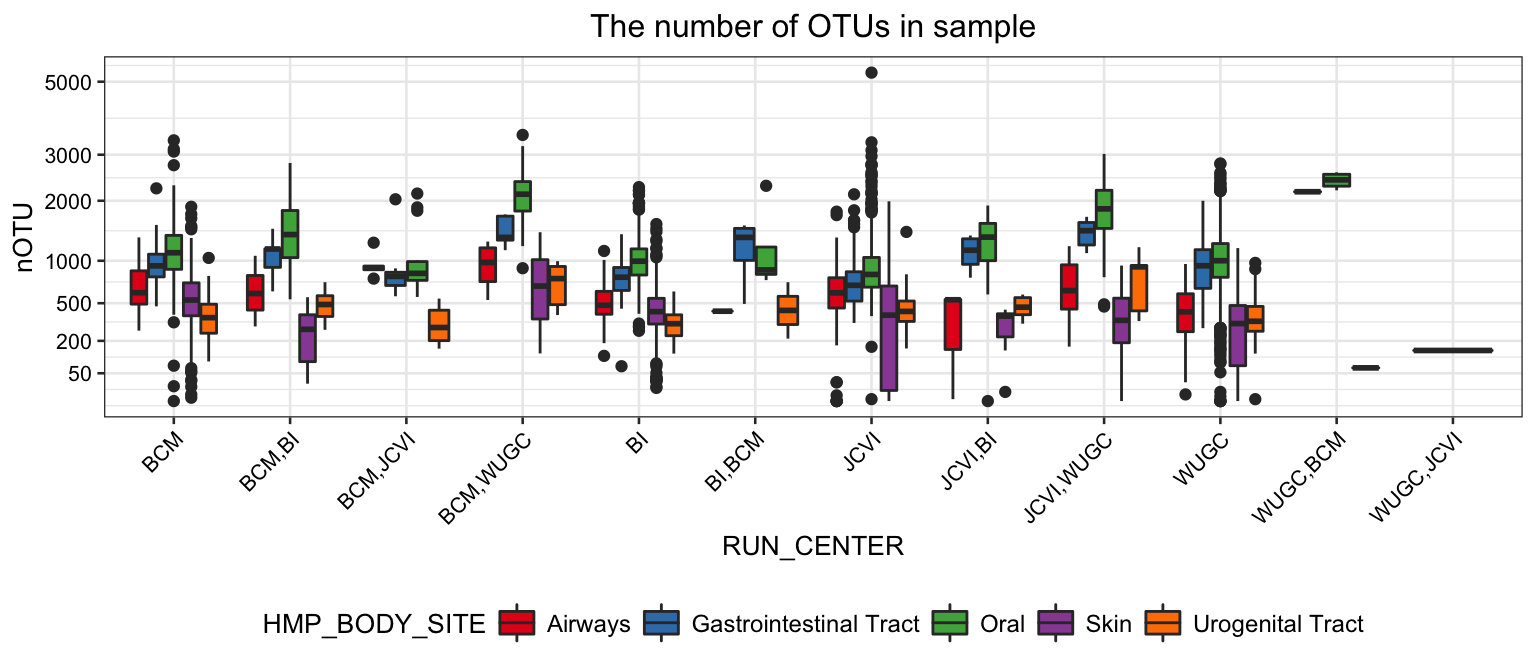
\includegraphics{figure/unnamed-chunk-50-1} \end{adjustwidth}

The sequencing depth of samples across different coordination centers are quite
similar. Within the coordination center, samples collected from \texttt{Skin} are more spread out in the sequencing depth than those from other body sites.

\begin{Shaded}
\begin{Highlighting}[]
\KeywordTok{ggplot}\NormalTok{(df_OTU) }\OperatorTok{+}
\StringTok{  }\KeywordTok{geom_boxplot}\NormalTok{(}\KeywordTok{aes}\NormalTok{(}\DataTypeTok{x =}\NormalTok{ RUN_CENTER, }\DataTypeTok{y =}\NormalTok{ Total_count,}
                   \DataTypeTok{block =}\NormalTok{ HMP_BODY_SITE, }\DataTypeTok{fill =}\NormalTok{ HMP_BODY_SITE)) }\OperatorTok{+}\StringTok{ }
\StringTok{  }\KeywordTok{scale_y_continuous}\NormalTok{(}\DataTypeTok{trans =} \KeywordTok{log2_trans}\NormalTok{()) }\OperatorTok{+}
\StringTok{  }\KeywordTok{labs}\NormalTok{(}\DataTypeTok{title =} \StringTok{"The sequencing depths of samples"}\NormalTok{) }\OperatorTok{+}
\StringTok{  }\KeywordTok{scale_fill_brewer}\NormalTok{(}\DataTypeTok{palette =} \StringTok{"Set1"}\NormalTok{) }\OperatorTok{+}
\StringTok{  }\NormalTok{prettify }
\end{Highlighting}
\end{Shaded}

\begin{adjustwidth}{\fltoffset}{0mm}
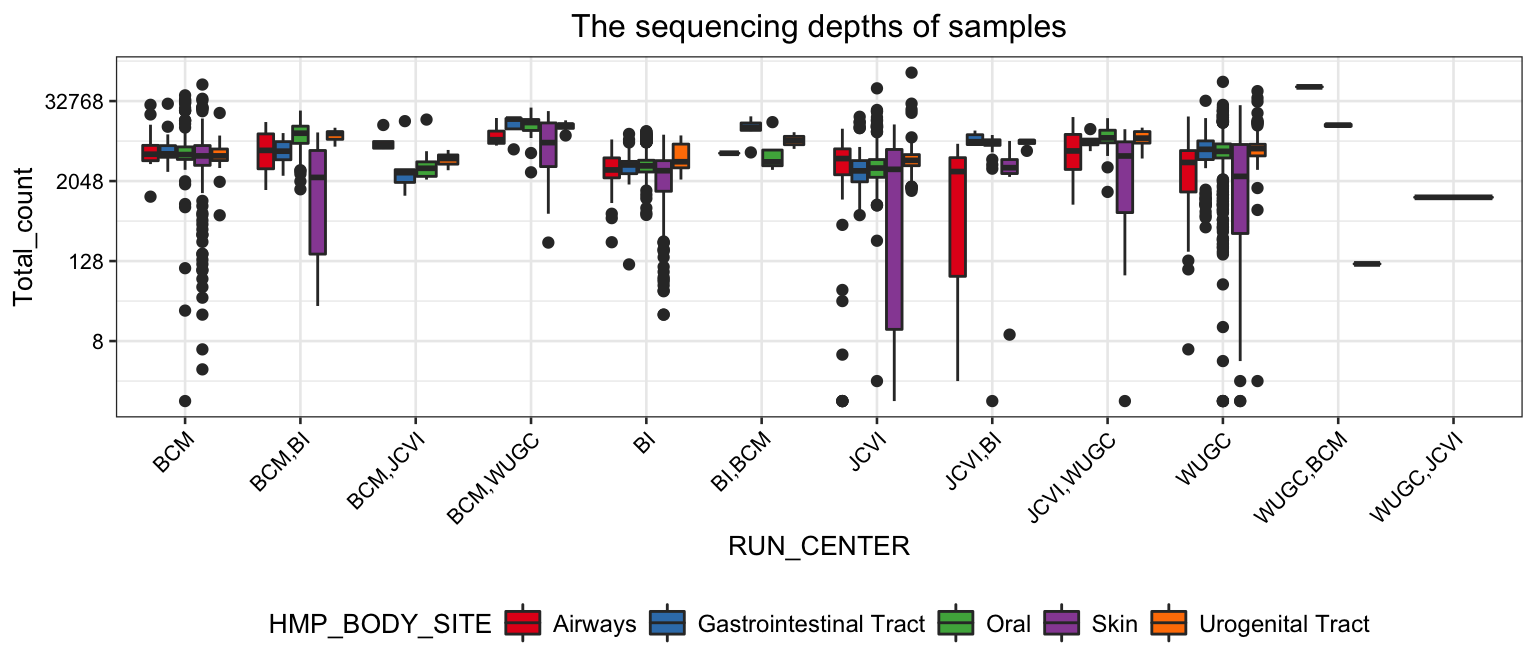
\includegraphics{figure/unnamed-chunk-51-1} \end{adjustwidth}

More samples are taken from the \texttt{oral} site than other body sites

\begin{Shaded}
\begin{Highlighting}[]
\KeywordTok{ggplot}\NormalTok{(df_OTU) }\OperatorTok{+}
\StringTok{  }\KeywordTok{geom_bar}\NormalTok{(}\KeywordTok{aes}\NormalTok{(RUN_CENTER, }\DataTypeTok{fill =}\NormalTok{ HMP_BODY_SITE),}
           \DataTypeTok{position =} \KeywordTok{position_dodge}\NormalTok{()) }\OperatorTok{+}
\StringTok{  }\KeywordTok{labs}\NormalTok{(}\DataTypeTok{title =} \StringTok{"The number of samples across centers"}\NormalTok{) }\OperatorTok{+}
\StringTok{  }\KeywordTok{scale_fill_brewer}\NormalTok{(}\DataTypeTok{palette =} \StringTok{"Set1"}\NormalTok{) }\OperatorTok{+}
\StringTok{  }\NormalTok{prettify }
\end{Highlighting}
\end{Shaded}

\begin{adjustwidth}{\fltoffset}{0mm}
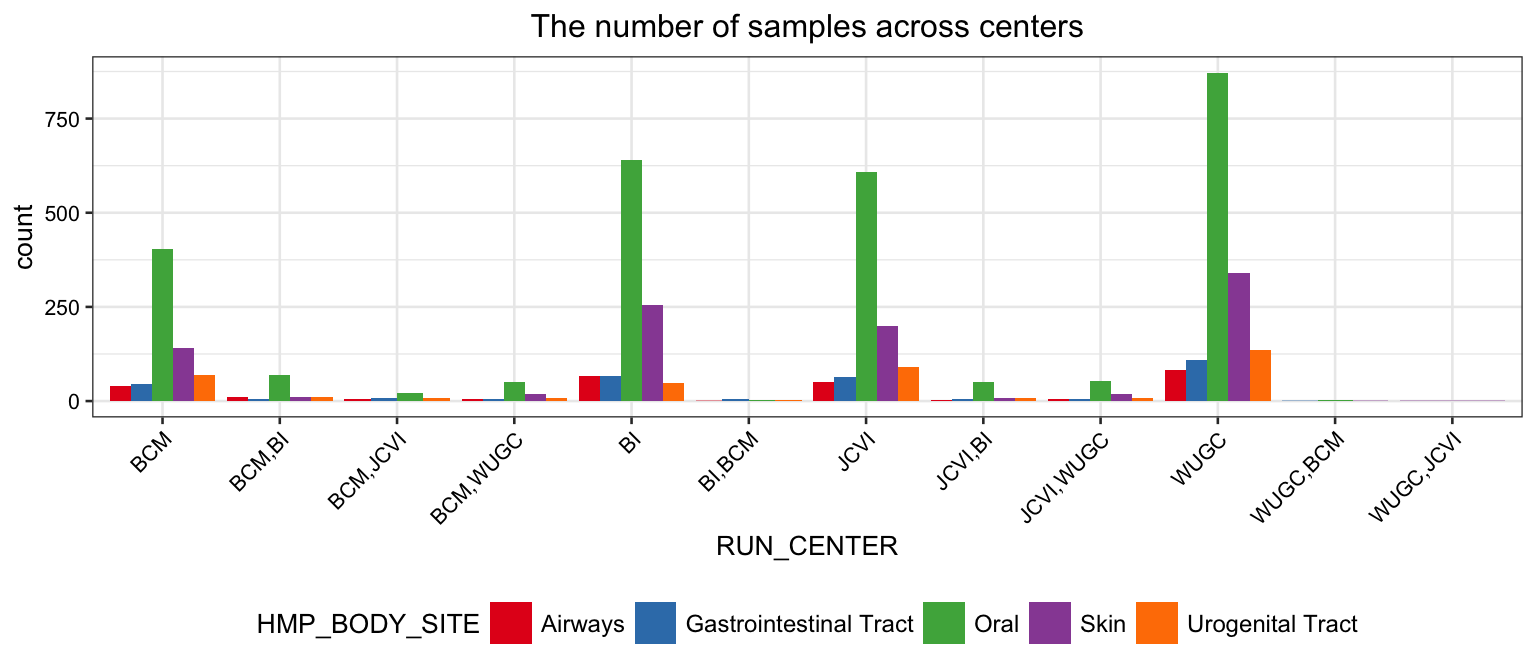
\includegraphics{figure/unnamed-chunk-52-1} \end{adjustwidth}

\hypertarget{the-relative-abundance-of-phyla-in-samples}{%
\subsection{The relative abundance of phyla in samples}\label{the-relative-abundance-of-phyla-in-samples}}

The relative abundance of OTUs within sample are calculated and stored in the \texttt{assays} with the name \texttt{rel\_abund}.

\begin{Shaded}
\begin{Highlighting}[]
\CommentTok{# add relative abundance in the second assays}
\NormalTok{abd <-}\StringTok{ }\KeywordTok{assays}\NormalTok{(tse_tax)[[}\DecValTok{1}\NormalTok{]]}
\KeywordTok{assays}\NormalTok{(tse_tax)[[}\StringTok{"rel_abund"}\NormalTok{]] <-}\StringTok{ }\KeywordTok{apply}\NormalTok{(abd, }\DecValTok{2}\NormalTok{, }\DataTypeTok{FUN =} \ControlFlowTok{function}\NormalTok{(x)\{}
\NormalTok{  x}\OperatorTok{/}\KeywordTok{sum}\NormalTok{(x)}
\NormalTok{\})}
\end{Highlighting}
\end{Shaded}

We aggregate the relative abundance to the phylum level using \texttt{aggValue}. It calculate the relative abundance of a phylum as the sum of the relative abundance of OTUs belonging to it.

\begin{Shaded}
\begin{Highlighting}[]
\CommentTok{# aggregation to the phylum level}
\NormalTok{lab <-}\StringTok{ }\KeywordTok{c}\NormalTok{(}\KeywordTok{rowTree}\NormalTok{(tse_tax)}\OperatorTok{$}\NormalTok{node.label, }\KeywordTok{rowTree}\NormalTok{(tse_tax)}\OperatorTok{$}\NormalTok{tip.label)}
\NormalTok{lab_phylum <-}\StringTok{ }\NormalTok{lab[}\KeywordTok{startsWith}\NormalTok{(lab, }\StringTok{"PHYLUM"}\NormalTok{)]}
\NormalTok{agg_phylum <-}\StringTok{ }\KeywordTok{aggValue}\NormalTok{(}\DataTypeTok{x =}\NormalTok{ tse_tax, }
                  \DataTypeTok{rowLevel =}\NormalTok{ lab_phylum,}
                  \DataTypeTok{assay =} \StringTok{"rel_abund"}\NormalTok{,}
                  \DataTypeTok{message =} \OtherTok{FALSE}\NormalTok{)}
\end{Highlighting}
\end{Shaded}

To compare the relative abundance of phyla across body sites, we average them over samples from the same body site, and show those with relative abundance above \(0.01\) in the scale \([0, 1]\).

\begin{Shaded}
\begin{Highlighting}[]
\NormalTok{aC <-}\StringTok{ }\KeywordTok{assays}\NormalTok{(agg_phylum)}\OperatorTok{$}\NormalTok{rel_abund}
\NormalTok{rD <-}\StringTok{ }\KeywordTok{rowData}\NormalTok{(agg_phylum) }
\NormalTok{cD <-}\StringTok{ }\KeywordTok{colData}\NormalTok{(agg_phylum) }
\NormalTok{rL <-}\StringTok{ }\KeywordTok{rowLinks}\NormalTok{(agg_phylum)}
\NormalTok{df_abd <-}\StringTok{ }\KeywordTok{t}\NormalTok{(aC) }\OperatorTok
\StringTok{  }\KeywordTok{data.frame}\NormalTok{() }\OperatorTok\StringTok{ }
\StringTok{  }\KeywordTok{mutate}\NormalTok{(}\DataTypeTok{body_site =}\NormalTok{ cD}\OperatorTok{$}\NormalTok{HMP_BODY_SITE,}
         \DataTypeTok{sample_id =} \KeywordTok{colnames}\NormalTok{(aC)) }\OperatorTok
\StringTok{  }\KeywordTok{gather}\NormalTok{(}\DataTypeTok{key =} \StringTok{"node"}\NormalTok{, }\DataTypeTok{value =} \StringTok{"rel_abund"}\NormalTok{, }
         \OperatorTok{-}\KeywordTok{c}\NormalTok{(body_site, sample_id)) }\OperatorTok
\StringTok{  }\KeywordTok{group_by}\NormalTok{(body_site, node) }\OperatorTok
\StringTok{  }\KeywordTok{summarize}\NormalTok{(}\DataTypeTok{relative_abundance =} \KeywordTok{mean}\NormalTok{(rel_abund)) }\OperatorTok
\StringTok{  }\KeywordTok{mutate}\NormalTok{(}\DataTypeTok{Phylum =}\NormalTok{ rD}\OperatorTok{$}\NormalTok{PHYLUM)}

\CommentTok{# The phylum level}
\KeywordTok{ggplot}\NormalTok{(df_abd) }\OperatorTok{+}
\StringTok{  }\KeywordTok{geom_bar}\NormalTok{(}\DataTypeTok{data =}\NormalTok{ . }\OperatorTok\StringTok{ }\KeywordTok{filter}\NormalTok{(relative_abundance }\OperatorTok{>=}\StringTok{ }\FloatTok{0.01}\NormalTok{),}
           \KeywordTok{aes}\NormalTok{(}\DataTypeTok{x=}\NormalTok{ body_site, }\DataTypeTok{y =}\NormalTok{ relative_abundance, }\DataTypeTok{fill =}\NormalTok{ Phylum),}
           \DataTypeTok{stat =} \StringTok{"identity"}\NormalTok{) }\OperatorTok{+}
\StringTok{  }\KeywordTok{scale_fill_brewer}\NormalTok{(}\DataTypeTok{palette =} \StringTok{"Set1"}\NormalTok{) }\OperatorTok{+}
\StringTok{  }\NormalTok{prettify}
\end{Highlighting}
\end{Shaded}

\begin{adjustwidth}{\fltoffset}{0mm}
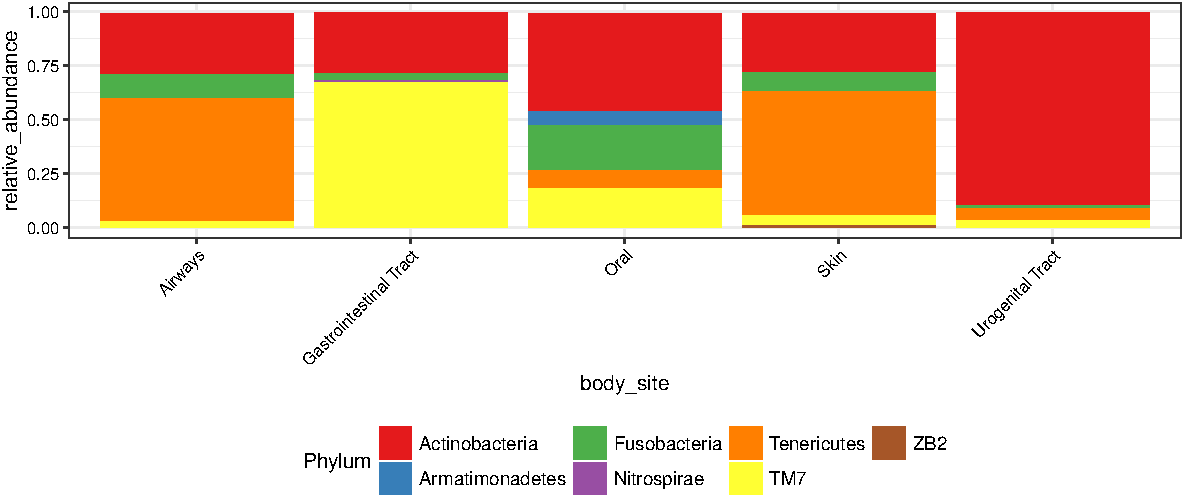
\includegraphics{figure/unnamed-chunk-55-1} \end{adjustwidth}

\hypertarget{dimensionality-reduction}{%
\subsection{Dimensionality reduction}\label{dimensionality-reduction}}

We visualize samples in reduced dimensions to see whether those from the same body site are more similar. Three dimensionality reduction techniques, including principal component analysis (PCA), t-distributed Stochastic Neighbor Embedding (t-SNE), uniform manifold approximation and projection (UMAP) are used. As \texttt{TreeSummarizedExperiment} is inherited from \texttt{SingleCellExperiment}, we could directly use functions from the package \emph{\href{https://bioconductor.org/packages/3.11/scater}{scater}}. We first apply techniques using data at the OTU level, then we further try t-SNE using data at different taxonomic levels, e.g., the genus and the phylum levels, to see whether the resolution affects the separation of samples.

\hypertarget{pca}{%
\subsubsection{PCA}\label{pca}}

The PCA is performed on the log-transformed counts that are stored in the \texttt{assays} table with the name \texttt{logcounts}. We see that the \texttt{Oral} samples are distinct from those of other body sites. Samples from \texttt{Skin}, \texttt{Urogenital Tract}, \texttt{Airways} and \texttt{Gastrointestinal Tract} are not separated very well in the top two principle components of PCA.

\begin{Shaded}
\begin{Highlighting}[]

\CommentTok{# log-transformed data}
\KeywordTok{assays}\NormalTok{(tse_tax)}\OperatorTok{$}\NormalTok{logcounts <-}\StringTok{ }\KeywordTok{log}\NormalTok{(}\KeywordTok{assays}\NormalTok{(tse_tax)[[}\DecValTok{1}\NormalTok{]] }\OperatorTok{+}\StringTok{ }\DecValTok{1}\NormalTok{)}

\CommentTok{# run PCA at the OTU level}
\NormalTok{tse_tax <-}\StringTok{ }\KeywordTok{runPCA}\NormalTok{(tse_tax, }\DataTypeTok{name=}\StringTok{"PCA_OTU"}\NormalTok{, }\DataTypeTok{exprs_values =} \StringTok{"logcounts"}\NormalTok{)}

\CommentTok{# plot samples in the reduced dimensions}
\KeywordTok{plotReducedDim}\NormalTok{(tse_tax, }\DataTypeTok{dimred =} \StringTok{"PCA_OTU"}\NormalTok{, }
               \DataTypeTok{colour_by =} \StringTok{"HMP_BODY_SITE"}\NormalTok{)}\OperatorTok{+}
\StringTok{  }\KeywordTok{labs}\NormalTok{(}\DataTypeTok{title =} \StringTok{"PCA at the OTU level"}\NormalTok{) }\OperatorTok{+}
\StringTok{  }\KeywordTok{guides}\NormalTok{(}\DataTypeTok{fill =} \KeywordTok{guide_legend}\NormalTok{(}\DataTypeTok{override.aes =} \KeywordTok{list}\NormalTok{(}\DataTypeTok{size=}\FloatTok{2.5}\NormalTok{, }\DataTypeTok{alpha =} \DecValTok{1}\NormalTok{))) }\OperatorTok{+}
\StringTok{  }\KeywordTok{theme}\NormalTok{(}\DataTypeTok{plot.title =} \KeywordTok{element_text}\NormalTok{(}\DataTypeTok{hjust =} \FloatTok{0.5}\NormalTok{),}
        \DataTypeTok{legend.position =} \StringTok{"bottom"}\NormalTok{)}
\end{Highlighting}
\end{Shaded}

\begin{adjustwidth}{\fltoffset}{0mm}
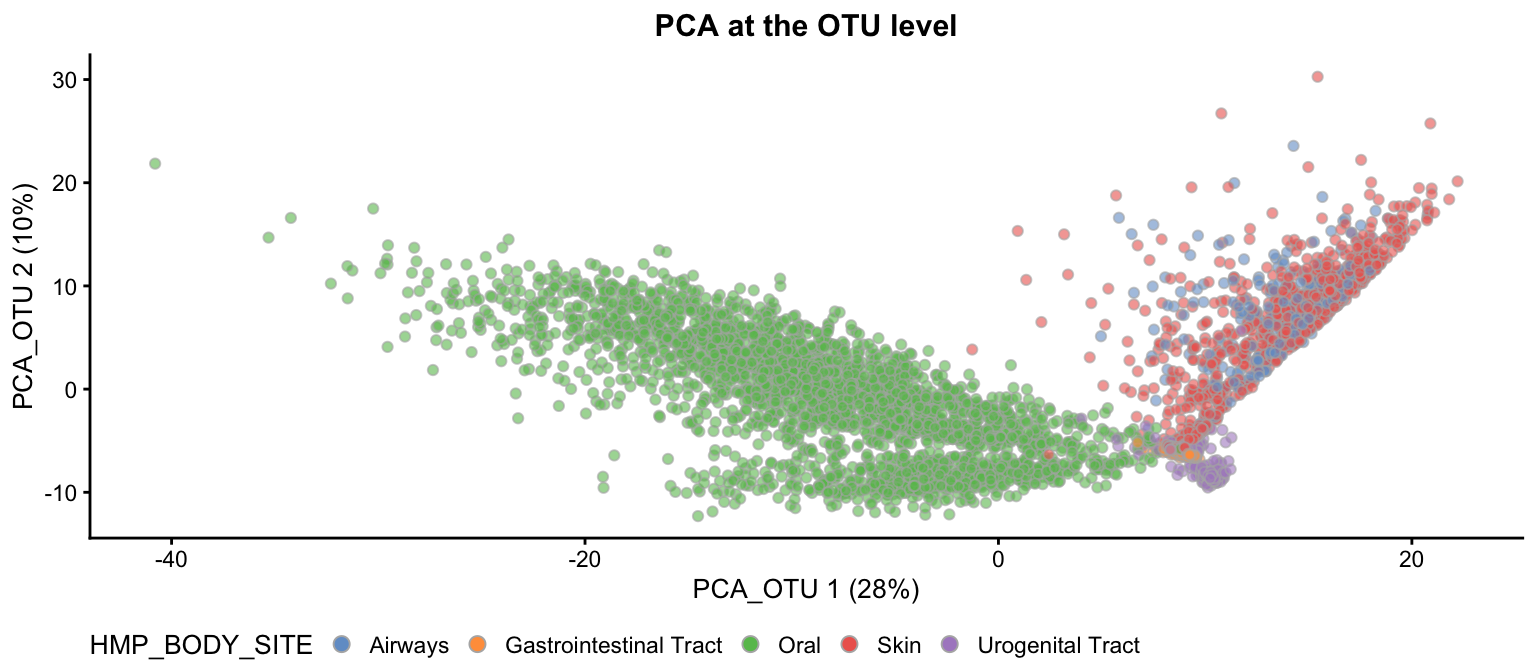
\includegraphics{figure/unnamed-chunk-56-1} \end{adjustwidth}

\hypertarget{t-sne}{%
\subsubsection{t-SNE}\label{t-sne}}

The separation is well improved with the use of \texttt{t-SNE}. Samples from \texttt{Oral}, \texttt{Gastrointestinal Tract}, and \texttt{Urogenital Tract} are in distinct clusters. Skin samples and airways samples still overlap.

\begin{Shaded}
\begin{Highlighting}[]

\CommentTok{# run PCA at the OTU level}
\NormalTok{tse_tax <-}\StringTok{ }\KeywordTok{runTSNE}\NormalTok{(tse_tax, }\DataTypeTok{name=}\StringTok{"TSNE_OTU"}\NormalTok{)}

\CommentTok{# plot samples in the reduced dimensions}
\NormalTok{tsne_otu <-}\StringTok{ }\KeywordTok{plotReducedDim}\NormalTok{(tse_tax, }\DataTypeTok{dimred =} \StringTok{"TSNE_OTU"}\NormalTok{, }
                           \DataTypeTok{colour_by =} \StringTok{"HMP_BODY_SITE"}\NormalTok{) }\OperatorTok{+}
\StringTok{  }\KeywordTok{labs}\NormalTok{(}\DataTypeTok{title =} \StringTok{"Use the OTU level"}\NormalTok{) }\OperatorTok{+}
\StringTok{  }\KeywordTok{theme}\NormalTok{(}\DataTypeTok{plot.title =} \KeywordTok{element_text}\NormalTok{(}\DataTypeTok{hjust =} \FloatTok{0.5}\NormalTok{)) }\OperatorTok{+}
\StringTok{  }\KeywordTok{scale_fill_brewer}\NormalTok{(}\DataTypeTok{palette =} \StringTok{"Set1"}\NormalTok{) }\OperatorTok{+}
\StringTok{  }\KeywordTok{labs}\NormalTok{(}\DataTypeTok{fill =} \StringTok{"Body sites"}\NormalTok{) }\OperatorTok{+}
\StringTok{  }\KeywordTok{guides}\NormalTok{(}\DataTypeTok{fill =} \KeywordTok{guide_legend}\NormalTok{(}\DataTypeTok{override.aes =} \KeywordTok{list}\NormalTok{(}\DataTypeTok{size=}\FloatTok{2.5}\NormalTok{, }\DataTypeTok{alpha =} \DecValTok{1}\NormalTok{))) }\OperatorTok{+}
\StringTok{  }\KeywordTok{theme}\NormalTok{(}\DataTypeTok{plot.title =} \KeywordTok{element_text}\NormalTok{(}\DataTypeTok{hjust =} \FloatTok{0.5}\NormalTok{),}
        \DataTypeTok{legend.position =} \StringTok{"bottom"}\NormalTok{)}
\NormalTok{tsne_otu}
\end{Highlighting}
\end{Shaded}

\begin{adjustwidth}{\fltoffset}{0mm}
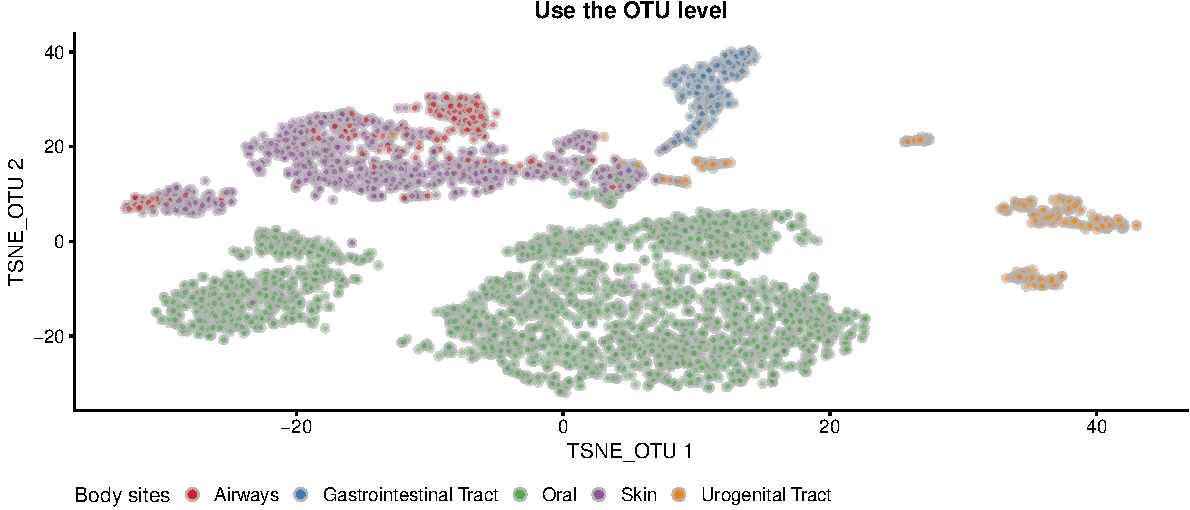
\includegraphics{figure/unnamed-chunk-57-1} \end{adjustwidth}

Notably, there are two well separated clusters belonging to oral samples. The small cluster includes samples from the \texttt{Supragingival Plaque} and \texttt{Subgingival Plaque}, and the other cluster includes samples from other oral sub-sites.

\begin{Shaded}
\begin{Highlighting}[]
\NormalTok{is_oral <-}\StringTok{ }\KeywordTok{colData}\NormalTok{(tse_tax)}\OperatorTok{$}\NormalTok{HMP_BODY_SITE }\OperatorTok\StringTok{ "Oral"}
\KeywordTok{colData}\NormalTok{(tse_tax)}\OperatorTok{$}\NormalTok{from_plaque <-}\StringTok{ }\KeywordTok{grepl}\NormalTok{(}\DataTypeTok{pattern =} \StringTok{"Plaque"}\NormalTok{, }
                                    \KeywordTok{colData}\NormalTok{(tse_tax)}\OperatorTok{$}\NormalTok{HMP_BODY_SUBSITE)}
\CommentTok{# Oral samples}
\KeywordTok{plotReducedDim}\NormalTok{(tse_tax[, is_oral], }\DataTypeTok{dimred =} \StringTok{"TSNE_OTU"}\NormalTok{,}
               \DataTypeTok{colour_by =} \StringTok{"from_plaque"}\NormalTok{) }\OperatorTok{+}
\StringTok{  }\KeywordTok{labs}\NormalTok{(}\DataTypeTok{title =} \StringTok{"OTU"}\NormalTok{) }\OperatorTok{+}
\StringTok{  }\KeywordTok{guides}\NormalTok{(}\DataTypeTok{fill =} \KeywordTok{guide_legend}\NormalTok{(}\DataTypeTok{override.aes =} \KeywordTok{list}\NormalTok{(}\DataTypeTok{size=}\FloatTok{2.5}\NormalTok{, }\DataTypeTok{alpha =} \DecValTok{1}\NormalTok{))) }\OperatorTok{+}
\StringTok{  }\KeywordTok{theme}\NormalTok{(}\DataTypeTok{plot.title =} \KeywordTok{element_text}\NormalTok{(}\DataTypeTok{hjust =} \FloatTok{0.5}\NormalTok{),}
        \DataTypeTok{legend.position =} \StringTok{"bottom"}\NormalTok{)}
\end{Highlighting}
\end{Shaded}

\begin{adjustwidth}{\fltoffset}{0mm}
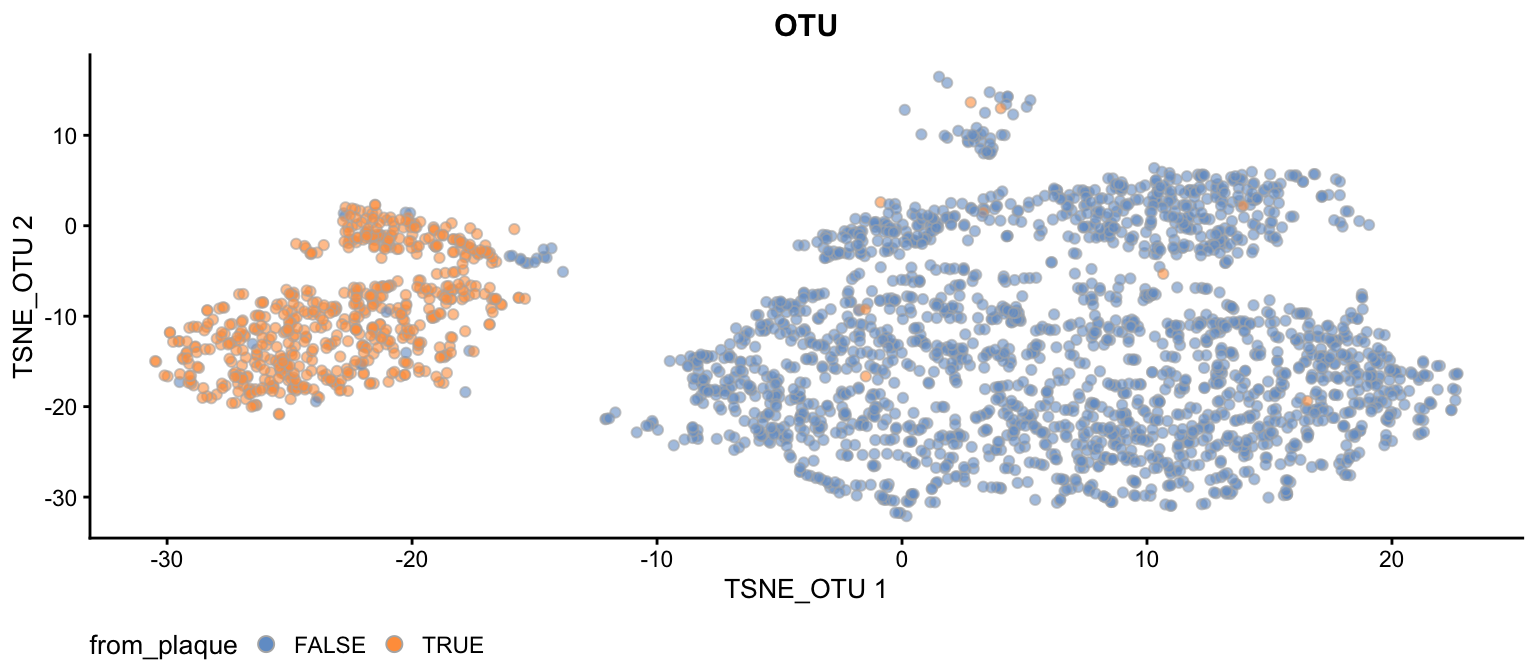
\includegraphics{figure/unnamed-chunk-58-1} \end{adjustwidth}

The separation of samples from different body sites become worse when the data on broader resolution is used.

\begin{Shaded}
\begin{Highlighting}[]
\CommentTok{# aggregation data to all internal nodes}
\NormalTok{tse_agg <-}\StringTok{ }\KeywordTok{aggValue}\NormalTok{(}\DataTypeTok{x =}\NormalTok{ tse_tax, }
                    \DataTypeTok{rowLevel =}\NormalTok{ tax_tree}\OperatorTok{$}\NormalTok{node.label,}
                    \DataTypeTok{assay =} \StringTok{"16SrRNA"}\NormalTok{,}
                    \DataTypeTok{message =} \OtherTok{FALSE}\NormalTok{)}
\CommentTok{# log-transform count }
\KeywordTok{assays}\NormalTok{(tse_agg)}\OperatorTok{$}\NormalTok{logcounts <-}\StringTok{ }\KeywordTok{log}\NormalTok{(}\KeywordTok{assays}\NormalTok{(tse_agg)[[}\DecValTok{1}\NormalTok{]] }\OperatorTok{+}\StringTok{ }\DecValTok{1}\NormalTok{)}
\end{Highlighting}
\end{Shaded}

\begin{Shaded}
\begin{Highlighting}[]
\NormalTok{tax_rank <-}\StringTok{ }\KeywordTok{c}\NormalTok{(}\StringTok{"GENUS"}\NormalTok{, }\StringTok{"FAMILY"}\NormalTok{, }\StringTok{"ORDER"}\NormalTok{, }\StringTok{"CLASS"}\NormalTok{, }\StringTok{"PHYLUM"}\NormalTok{)}
\KeywordTok{names}\NormalTok{(tax_rank) <-}\StringTok{ }\NormalTok{tax_rank}
\NormalTok{fig_list <-}\StringTok{ }\KeywordTok{lapply}\NormalTok{(tax_rank, }\DataTypeTok{FUN =} \ControlFlowTok{function}\NormalTok{(x) \{}
\NormalTok{  xx <-}\StringTok{ }\KeywordTok{startsWith}\NormalTok{(}\KeywordTok{rowLinks}\NormalTok{(tse_agg)}\OperatorTok{$}\NormalTok{nodeLab, x)}
\NormalTok{  xx_tse <-}\StringTok{ }\KeywordTok{runTSNE}\NormalTok{(tse_agg, }\DataTypeTok{name =} \KeywordTok{paste0}\NormalTok{(}\StringTok{"TSNE_"}\NormalTok{, x), }
                    \DataTypeTok{exprs_values =} \StringTok{"logcounts"}\NormalTok{,}
                    \DataTypeTok{subset_row =} \KeywordTok{rownames}\NormalTok{(tse_agg)[xx])}

  \CommentTok{# plot samples in the reduced dimensions}
  \KeywordTok{plotReducedDim}\NormalTok{(xx_tse, }\DataTypeTok{dimred =} \KeywordTok{paste0}\NormalTok{(}\StringTok{"TSNE_"}\NormalTok{, x),}
                 \DataTypeTok{colour_by =} \StringTok{"HMP_BODY_SITE"}\NormalTok{) }\OperatorTok{+}
\StringTok{    }\KeywordTok{labs}\NormalTok{(}\DataTypeTok{title =} \KeywordTok{paste0}\NormalTok{(}\StringTok{"Use the "}\NormalTok{, x, }\StringTok{" level"}\NormalTok{)) }\OperatorTok{+}
\StringTok{    }\KeywordTok{theme}\NormalTok{(}\DataTypeTok{plot.title =} \KeywordTok{element_text}\NormalTok{(}\DataTypeTok{hjust =} \FloatTok{0.5}\NormalTok{))}\OperatorTok{+}
\StringTok{    }\KeywordTok{scale_fill_brewer}\NormalTok{(}\DataTypeTok{palette =} \StringTok{"Set1"}\NormalTok{) }\OperatorTok{+}\StringTok{ }
\StringTok{    }\KeywordTok{theme}\NormalTok{(}\DataTypeTok{legend.position =} \StringTok{"none"}\NormalTok{) }\OperatorTok{+}
\StringTok{  }\KeywordTok{guides}\NormalTok{(}\DataTypeTok{fill =} \KeywordTok{guide_legend}\NormalTok{(}\DataTypeTok{override.aes =} \KeywordTok{list}\NormalTok{(}\DataTypeTok{size=}\FloatTok{2.5}\NormalTok{)))}
\NormalTok{\})}
\end{Highlighting}
\end{Shaded}

\begin{Shaded}
\begin{Highlighting}[]
\NormalTok{legend <-}\StringTok{ }\KeywordTok{get_legend}\NormalTok{(}
  \CommentTok{# create some space to the left of the legend}
\NormalTok{  tsne_otu }\OperatorTok{+}\StringTok{ }
\StringTok{    }\KeywordTok{theme}\NormalTok{(}\DataTypeTok{legend.box.margin =} \KeywordTok{margin}\NormalTok{(}\DecValTok{0}\NormalTok{, }\DecValTok{0}\NormalTok{, }\DecValTok{0}\NormalTok{, }\DecValTok{35}\NormalTok{),}
          \DataTypeTok{legend.position =} \StringTok{"right"}\NormalTok{)}
\NormalTok{  )}
\KeywordTok{plot_grid}\NormalTok{(}\DataTypeTok{plotlist =}\NormalTok{ fig_list,}
\NormalTok{          legend, }\DataTypeTok{nrow =} \DecValTok{2}\NormalTok{)}
\end{Highlighting}
\end{Shaded}

\begin{adjustwidth}{\fltoffset}{0mm}
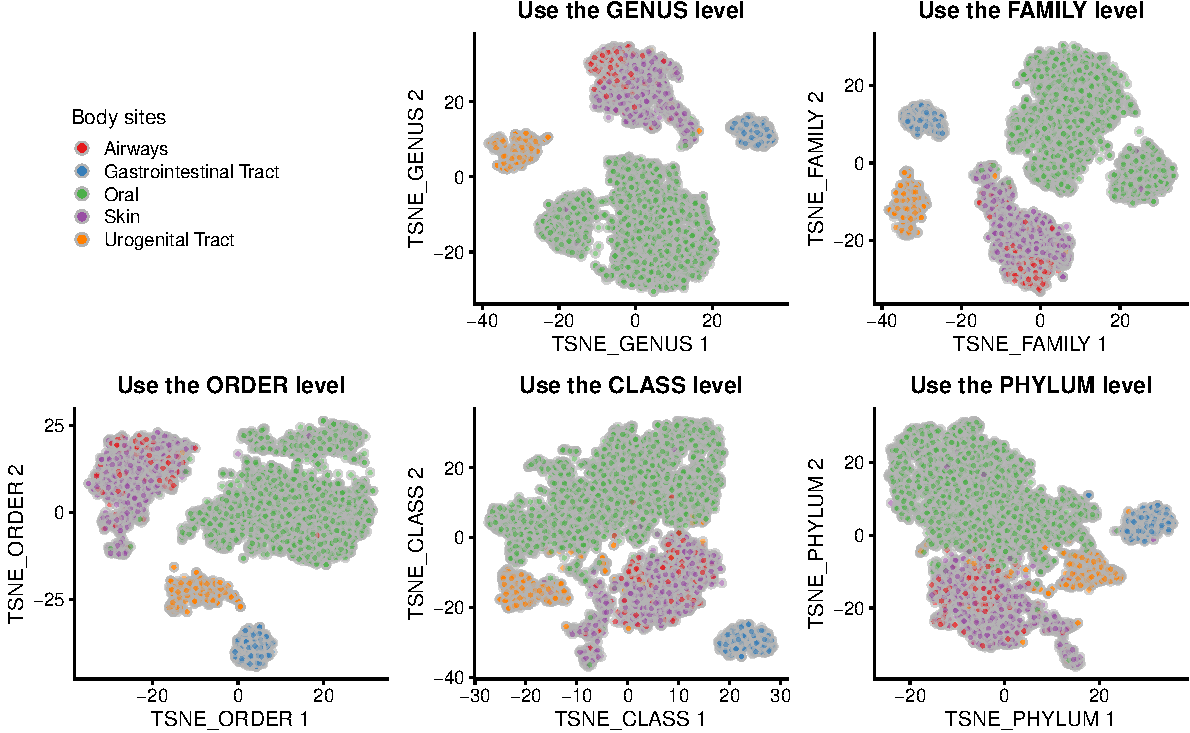
\includegraphics[width=1\linewidth,]{figure/unnamed-chunk-61-1} \end{adjustwidth}

\hypertarget{umap}{%
\subsubsection{UMAP}\label{umap}}

\begin{Shaded}
\begin{Highlighting}[]
\CommentTok{# run UMAP at the OTU level}
\NormalTok{tse_tax <-}\StringTok{ }\KeywordTok{runUMAP}\NormalTok{(tse_tax, }\DataTypeTok{name=}\StringTok{"UMAP_OTU"}\NormalTok{)}

\CommentTok{# plot samples in the reduced dimensions}
\KeywordTok{plotReducedDim}\NormalTok{(tse_tax, }\DataTypeTok{dimred =} \StringTok{"UMAP_OTU"}\NormalTok{, }
               \DataTypeTok{colour_by =} \StringTok{"HMP_BODY_SITE"}\NormalTok{) }\OperatorTok{+}
\StringTok{  }\KeywordTok{labs}\NormalTok{(}\DataTypeTok{title =} \StringTok{"UMAP at the OTU level"}\NormalTok{) }\OperatorTok{+}
\StringTok{  }\KeywordTok{guides}\NormalTok{(}\DataTypeTok{fill =} \KeywordTok{guide_legend}\NormalTok{(}\DataTypeTok{override.aes =} \KeywordTok{list}\NormalTok{(}\DataTypeTok{size=}\FloatTok{2.5}\NormalTok{, }\DataTypeTok{alpha =} \DecValTok{1}\NormalTok{))) }\OperatorTok{+}
\StringTok{  }\KeywordTok{theme}\NormalTok{(}\DataTypeTok{plot.title =} \KeywordTok{element_text}\NormalTok{(}\DataTypeTok{hjust =} \FloatTok{0.5}\NormalTok{),}
        \DataTypeTok{legend.position =} \StringTok{"bottom"}\NormalTok{)}
\end{Highlighting}
\end{Shaded}

\begin{adjustwidth}{\fltoffset}{0mm}
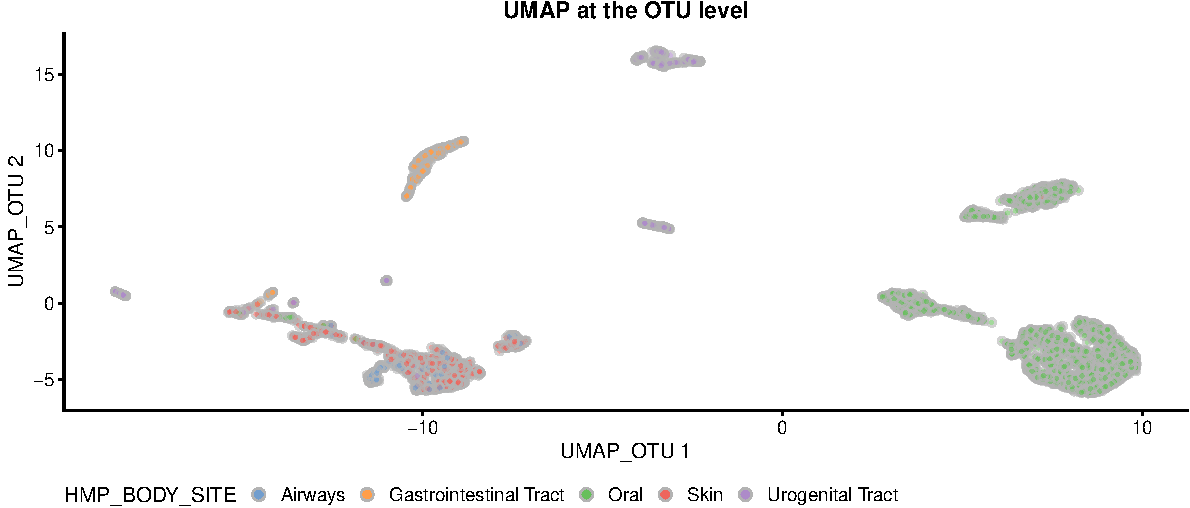
\includegraphics{figure/unnamed-chunk-62-1} \end{adjustwidth}

\hypertarget{fliter-samples-and-otus}{%
\subsection{Fliter samples and OTUs}\label{fliter-samples-and-otus}}

When preprocessing data, we might want to remove some samples or OTUs for some reasons. For example, if we are only interested in \texttt{Stool} and \texttt{Throat} samples provided by the center \texttt{BCM}.

\begin{Shaded}
\begin{Highlighting}[]
\NormalTok{count <-}\StringTok{ }\KeywordTok{assays}\NormalTok{(tse_tax)[[}\DecValTok{1}\NormalTok{]]}
\NormalTok{df_BCM <-}\StringTok{ }\KeywordTok{colData}\NormalTok{(tse_tax) }\OperatorTok
\StringTok{  }\KeywordTok{data.frame}\NormalTok{() }\OperatorTok
\StringTok{  }\KeywordTok{mutate}\NormalTok{(}\DataTypeTok{nOTU =} \KeywordTok{colSums}\NormalTok{(count }\OperatorTok{>}\StringTok{ }\DecValTok{0}\NormalTok{),}
         \DataTypeTok{Total_count =} \KeywordTok{colSums}\NormalTok{(count)) }\OperatorTok
\StringTok{  }\KeywordTok{mutate}\NormalTok{(}\DataTypeTok{index_sample =} \KeywordTok{row_number}\NormalTok{()) }\OperatorTok
\StringTok{  }\NormalTok{dplyr}\OperatorTok{::}\KeywordTok{filter}\NormalTok{(RUN_CENTER }\OperatorTok\StringTok{ "BCM"}\NormalTok{) }\OperatorTok
\StringTok{  }\NormalTok{dplyr}\OperatorTok{::}\KeywordTok{filter}\NormalTok{(HMP_BODY_SUBSITE }\OperatorTok\StringTok{ }\KeywordTok{c}\NormalTok{(}\StringTok{"Stool"}\NormalTok{, }\StringTok{"Throat"}\NormalTok{)) }
\end{Highlighting}
\end{Shaded}

We further remove samples that have relatively lower number of OTUs (\(<200\)) and sequencing depths (\(<2050\)).

\begin{Shaded}
\begin{Highlighting}[]
\CommentTok{# The number of OTUs  V.S. The sequencing depth}
\KeywordTok{ggplot}\NormalTok{(df_BCM) }\OperatorTok{+}
\StringTok{  }\KeywordTok{geom_point}\NormalTok{(}\KeywordTok{aes}\NormalTok{(}\DataTypeTok{x =}\NormalTok{ nOTU, }\DataTypeTok{y =}\NormalTok{ Total_count,}
                \DataTypeTok{color =}\NormalTok{ HMP_BODY_SUBSITE))}\OperatorTok{+}\StringTok{ }
\StringTok{  }\KeywordTok{scale_x_sqrt}\NormalTok{(}\DataTypeTok{breaks =} \KeywordTok{c}\NormalTok{(}\DecValTok{200}\NormalTok{, }\DecValTok{500}\NormalTok{, }\DecValTok{1000}\NormalTok{, }\DecValTok{2000}\NormalTok{, }\DecValTok{3000}\NormalTok{)) }\OperatorTok{+}
\StringTok{  }\KeywordTok{scale_y_sqrt}\NormalTok{(}\DataTypeTok{breaks =} \KeywordTok{c}\NormalTok{(}\DecValTok{2050}\NormalTok{, }\DecValTok{5000}\NormalTok{, }\DecValTok{10000}\NormalTok{, }\DecValTok{20000}\NormalTok{, }\DecValTok{30000}\NormalTok{)) }\OperatorTok{+}
\StringTok{  }\KeywordTok{labs}\NormalTok{(}\DataTypeTok{title =} \StringTok{"The number of non-zero nOTU VS. the sequencing depth"}\NormalTok{) }\OperatorTok{+}
\StringTok{  }\NormalTok{prettify }
\end{Highlighting}
\end{Shaded}

\begin{adjustwidth}{\fltoffset}{0mm}
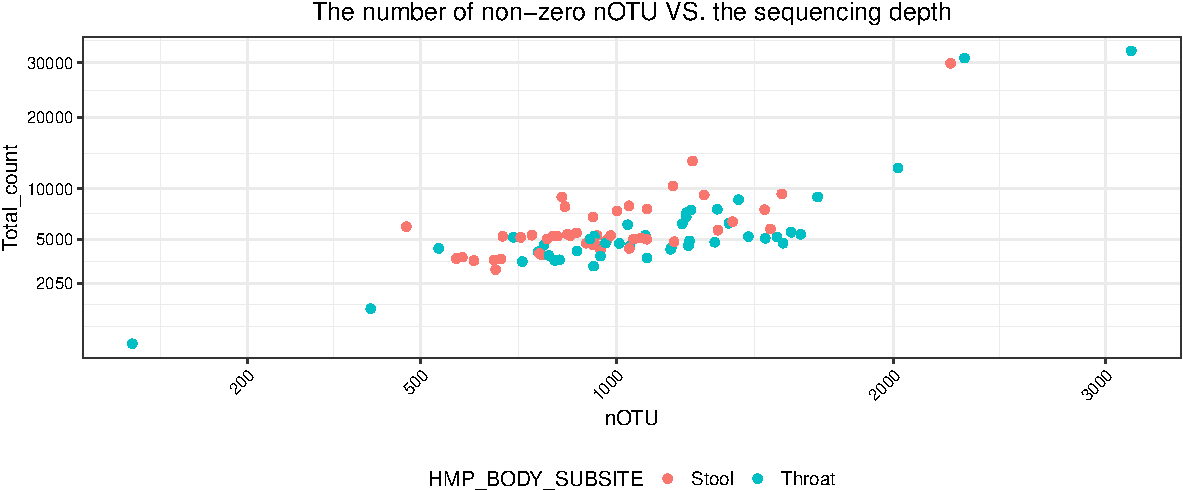
\includegraphics{figure/unnamed-chunk-64-1} \end{adjustwidth}

\begin{Shaded}
\begin{Highlighting}[]

\CommentTok{# samples that are kept}
\NormalTok{sel <-}\StringTok{ }\NormalTok{df_BCM }\OperatorTok
\StringTok{  }\NormalTok{dplyr}\OperatorTok{::}\KeywordTok{filter}\NormalTok{(nOTU }\OperatorTok{>}\StringTok{ }\DecValTok{200} \OperatorTok{&}\StringTok{ }\NormalTok{Total_count }\OperatorTok{>}\StringTok{ }\DecValTok{2050}\NormalTok{) }\OperatorTok
\StringTok{  }\KeywordTok{select}\NormalTok{(index_sample) }\OperatorTok
\StringTok{  }\KeywordTok{unlist}\NormalTok{()}

\NormalTok{tse_BCM <-}\StringTok{ }\NormalTok{tse_tax[, sel]}
\end{Highlighting}
\end{Shaded}

OTUs that appear in less than \(10%
\) of samples are removed, and their corresponding leaves on the tree are dropped.

\begin{Shaded}
\begin{Highlighting}[]
\CommentTok{# remove OTUs}
\NormalTok{count <-}\StringTok{ }\KeywordTok{assays}\NormalTok{(tse_BCM)[[}\DecValTok{1}\NormalTok{]]}
\NormalTok{isRare <-}\StringTok{ }\KeywordTok{rowSums}\NormalTok{(count}\OperatorTok{>}\DecValTok{0}\NormalTok{) }\OperatorTok{<}\StringTok{ }\FloatTok{0.1}\OperatorTok{*}\KeywordTok{ncol}\NormalTok{(tse_BCM)}
\NormalTok{tse_BCM <-}\StringTok{ }\NormalTok{tse_BCM[}\OperatorTok{!}\NormalTok{isRare, ]}

\CommentTok{# drop leaves of the removed OTUs from the tree}
\NormalTok{old_tree <-}\StringTok{ }\KeywordTok{rowTree}\NormalTok{(tse_BCM)}
\NormalTok{rmTip <-}\StringTok{ }\KeywordTok{setdiff}\NormalTok{(old_tree}\OperatorTok{$}\NormalTok{tip.label, }\KeywordTok{rowLinks}\NormalTok{(tse_BCM)}\OperatorTok{$}\NormalTok{nodeLab)}
\NormalTok{new_tree <-}\StringTok{ }\KeywordTok{drop.tip}\NormalTok{(}\DataTypeTok{phy =}\NormalTok{ old_tree, }\DataTypeTok{tip =}\NormalTok{ rmTip, }
                     \DataTypeTok{trim.internal =} \OtherTok{TRUE}\NormalTok{, }
                     \DataTypeTok{collapse.singles =} \OtherTok{FALSE}\NormalTok{)}

\CommentTok{# update the TreeSumamrizedExperiment}
\NormalTok{tse_BCM <-}\StringTok{ }\KeywordTok{changeTree}\NormalTok{(}\DataTypeTok{x =}\NormalTok{ tse_BCM, }\DataTypeTok{rowTree =}\NormalTok{ new_tree,}
                      \DataTypeTok{rowNodeLab =} \KeywordTok{rowData}\NormalTok{(tse_BCM)}\OperatorTok{$}\NormalTok{CONSENSUS_LINEAGE)}
\NormalTok{tse_BCM}
\CommentTok{## class: TreeSummarizedExperiment }
\CommentTok{## dim: 3243 88 }
\CommentTok{## metadata(1): experimentData}
\CommentTok{## assays(3): 16SrRNA rel_abund logcounts}
\CommentTok{## rownames(3243): OTU_97.10033 OTU_97.1005 ... OTU_97.997 OTU_97.9994}
\CommentTok{## rowData names(7): CONSENSUS_LINEAGE SUPERKINGDOM ... FAMILY GENUS}
\CommentTok{## colnames(88): 700013549 700016542 ... 700111985 700111996}
\CommentTok{## colData names(8): RSID VISITNO ... SRS_SAMPLE_ID from_plaque}
\CommentTok{## reducedDimNames(3): PCA_OTU TSNE_OTU UMAP_OTU}
\CommentTok{## altExpNames(0):}
\CommentTok{## rowLinks: a LinkDataFrame (3243 rows)}
\CommentTok{## rowTree: a phylo (96 leaves)}
\CommentTok{## colLinks: NULL}
\CommentTok{## colTree: NULL}
\end{Highlighting}
\end{Shaded}

\hypertarget{heatmap-at-different-taxonomic-levels}{%
\subsection{Heatmap at different taxonomic levels}\label{heatmap-at-different-taxonomic-levels}}

The relative abundance of taxa could be visualized at different taxonomic levels. At the phylum level, stool samples have higher \emph{Bacteroidetes} and lower \emph{Firmicutes} than throat samples. When visualizing data on a higher resolution (e.g., the genus level), heterogeneities are seen within the same phylum. For example, the \emph{Prevotella} has lower relative abundance in stool samples but \emph{Parabacteroides} is the other way around even they belong to the same phylum \emph{Bacterodetes}.

We first calculate the relative abundance of OTUs within the sample, and then aggregate to all internal nodes that represent taxa at different levels.

\begin{Shaded}
\begin{Highlighting}[]
\CommentTok{# store the relative abundance in a table of assays}
\KeywordTok{assays}\NormalTok{(tse_BCM)[[}\StringTok{"rel_abund"}\NormalTok{]] <-}\StringTok{ }\KeywordTok{apply}\NormalTok{(}\KeywordTok{assays}\NormalTok{(tse_BCM)[[}\DecValTok{1}\NormalTok{]], }\DecValTok{2}\NormalTok{, }
                                        \DataTypeTok{FUN =} \ControlFlowTok{function}\NormalTok{(x)\{}
\NormalTok{                                          x}\OperatorTok{/}\KeywordTok{sum}\NormalTok{(x)}
\NormalTok{                                        \})}

\CommentTok{# aggregation: all internal nodes}
\NormalTok{agg_BCM <-}\StringTok{ }\KeywordTok{aggValue}\NormalTok{(}\DataTypeTok{x =}\NormalTok{ tse_BCM, }
                    \DataTypeTok{rowLevel =} \KeywordTok{rowTree}\NormalTok{(tse_BCM)}\OperatorTok{$}\NormalTok{node.label, }
                    \DataTypeTok{FUN =}\NormalTok{ sum)}
\end{Highlighting}
\end{Shaded}

Nodes (\texttt{lab\_phylum}) representing taxa at the phylum level are obtained, and their relative abundances in different samples (\texttt{mat\_phylum}) are extracted.

\begin{Shaded}
\begin{Highlighting}[]
\CommentTok{# Extract the data at the phylum level}
\NormalTok{lab <-}\StringTok{ }\KeywordTok{c}\NormalTok{(}\KeywordTok{rowTree}\NormalTok{(agg_BCM)}\OperatorTok{$}\NormalTok{node.label, }\KeywordTok{rowTree}\NormalTok{(agg_BCM)}\OperatorTok{$}\NormalTok{tip.label)}
\NormalTok{lab_phylum <-}\StringTok{ }\NormalTok{lab[}\KeywordTok{startsWith}\NormalTok{(lab, }\StringTok{"PHYLUM"}\NormalTok{)]}
\NormalTok{mat_phylum <-}\StringTok{ }\NormalTok{agg_BCM }\OperatorTok\StringTok{ }
\StringTok{  }\KeywordTok{subsetByNode}\NormalTok{(}\DataTypeTok{rowNode =}\NormalTok{ lab_phylum) }\OperatorTok\StringTok{ }\NormalTok{assays }\OperatorTok
\StringTok{  }\KeywordTok{nth}\NormalTok{(}\DecValTok{2}\NormalTok{) }\OperatorTok
\StringTok{  }\KeywordTok{data.frame}\NormalTok{(}\DataTypeTok{check.names =} \OtherTok{FALSE}\NormalTok{)}
\end{Highlighting}
\end{Shaded}

Then, we plot the tree and label nodes representing phyla using
\emph{\href{https://bioconductor.org/packages/3.11/ggtree}{ggtree}}

\begin{Shaded}
\begin{Highlighting}[]
\CommentTok{# Plot the tree figure}
\NormalTok{treeFig <-}\StringTok{ }\KeywordTok{ggtree}\NormalTok{(}\KeywordTok{rowTree}\NormalTok{(agg_BCM), }\DataTypeTok{branch.length =} \StringTok{"none"}\NormalTok{, }
                  \DataTypeTok{color =} \StringTok{"grey"}\NormalTok{) }\OperatorTok{+}
\StringTok{  }\KeywordTok{geom_point2}\NormalTok{(}\KeywordTok{aes}\NormalTok{(}\DataTypeTok{subset =}\NormalTok{ label }\OperatorTok\StringTok{ }\NormalTok{lab_phylum), }
              \DataTypeTok{color =} \StringTok{"red"}\NormalTok{, }\DataTypeTok{size  =} \FloatTok{1.3}\NormalTok{) }\OperatorTok{+}
\StringTok{    }\KeywordTok{expand_limits}\NormalTok{(}\DataTypeTok{x =} \FloatTok{7.5}\NormalTok{)}

\NormalTok{clade_phylum <-}\StringTok{ }\KeywordTok{gsub}\NormalTok{(}\DataTypeTok{pattern =} \StringTok{".*:"}\NormalTok{, }\StringTok{""}\NormalTok{, lab_phylum)}
\NormalTok{node_phylum <-}\StringTok{ }\KeywordTok{transNode}\NormalTok{(}\DataTypeTok{tree =} \KeywordTok{rowTree}\NormalTok{(agg_BCM), }\DataTypeTok{node =}\NormalTok{ lab_phylum)}
\NormalTok{colrs <-}\StringTok{ }\KeywordTok{brewer_pal}\NormalTok{(}\DataTypeTok{palette =} \StringTok{"Set1"}\NormalTok{)(}\DecValTok{8}\NormalTok{)}
\ControlFlowTok{for}\NormalTok{ (i }\ControlFlowTok{in} \KeywordTok{seq_along}\NormalTok{(node_phylum)) \{}
\NormalTok{  treeFig <-}\StringTok{ }\NormalTok{treeFig }\OperatorTok{+}
\StringTok{    }\KeywordTok{geom_cladelabel}\NormalTok{(}\DataTypeTok{node  =}\NormalTok{ node_phylum[i], }\DataTypeTok{label =}\NormalTok{ clade_phylum[i],}
                    \DataTypeTok{fontsize =} \DecValTok{3}\NormalTok{, }\DataTypeTok{color =}\NormalTok{ colrs[i],}
                    \DataTypeTok{barsize =} \DecValTok{1}\NormalTok{) }
\NormalTok{\}}
\NormalTok{treeFig}
\end{Highlighting}
\end{Shaded}

\begin{adjustwidth}{\fltoffset}{0mm}
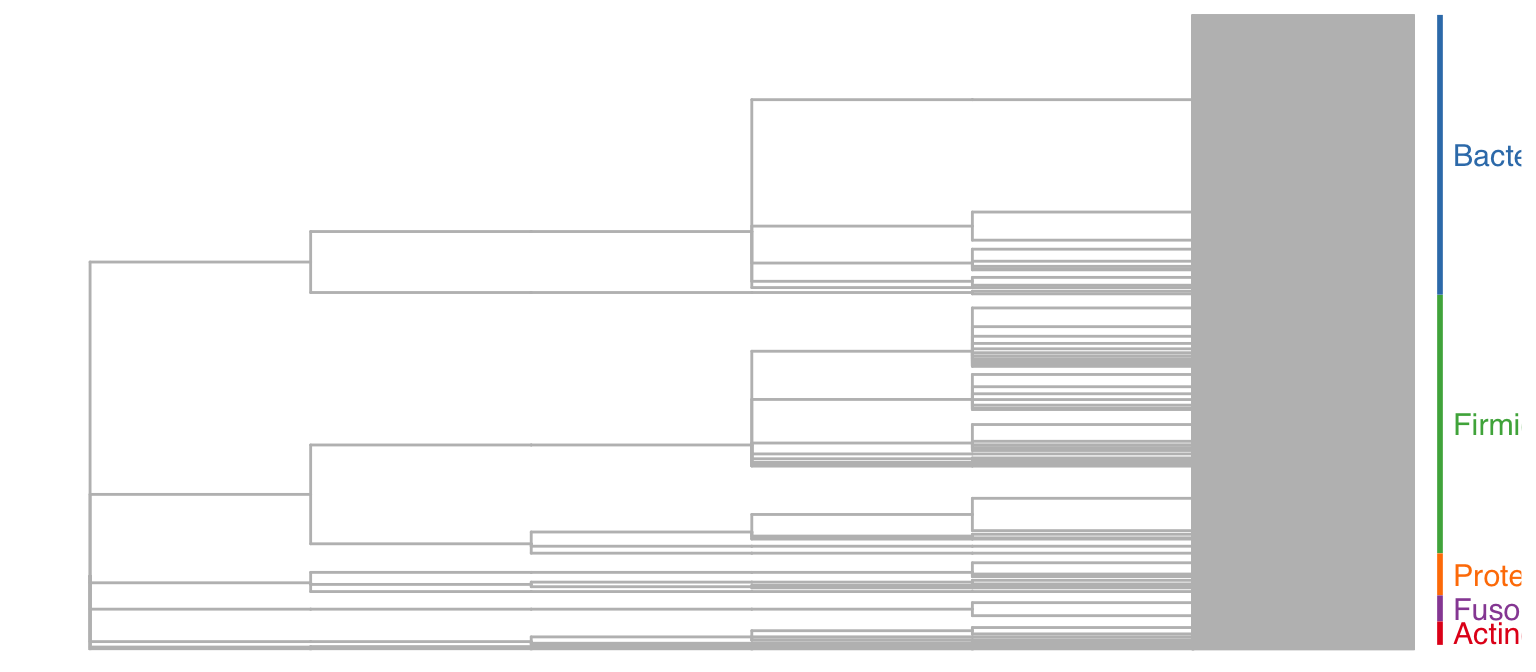
\includegraphics{figure/unnamed-chunk-68-1} \end{adjustwidth}

The relative abundance of phyla are visualized as a heatmap using \emph{\href{https://bioconductor.org/packages/3.11/TreeHeatmap}{TreeHeatmap}}. Samples from throat and stool are split as shown in Figure \ref{fig:treehm}.

\begin{Shaded}
\begin{Highlighting}[]
\CommentTok{# label the body subsites of samples}
\NormalTok{anno_c <-}\StringTok{ }\KeywordTok{setNames}\NormalTok{(}\KeywordTok{colData}\NormalTok{(agg_BCM)}\OperatorTok{$}\NormalTok{HMP_BODY_SUBSITE,}
                   \KeywordTok{rownames}\NormalTok{(}\KeywordTok{colData}\NormalTok{(agg_BCM)))}

\CommentTok{## align heatmap to the tree}
\NormalTok{fig1 <-}\StringTok{ }\KeywordTok{TreeHeatmap}\NormalTok{(}\DataTypeTok{tree =} \KeywordTok{rowTree}\NormalTok{(agg_BCM),}
            \DataTypeTok{hm_data =}\NormalTok{ mat_phylum, }
            \DataTypeTok{tree_fig =}\NormalTok{ treeFig, }
            \DataTypeTok{tree_hm_gap =} \DecValTok{5}\NormalTok{, }
            \DataTypeTok{column_split =}\NormalTok{ anno_c,}
            \DataTypeTok{column_anno =}\NormalTok{ anno_c, }
            \DataTypeTok{column_anno_color =} \KeywordTok{c}\NormalTok{(}\DataTypeTok{Stool =} \StringTok{"red"}\NormalTok{, }\DataTypeTok{Throat =} \StringTok{"blue"}\NormalTok{),}
            \DataTypeTok{column_anno_size =} \DecValTok{2}\NormalTok{,}
            \DataTypeTok{column_anno_gap =} \DecValTok{35}\NormalTok{)}
\NormalTok{fig1}
\end{Highlighting}
\end{Shaded}

\begin{adjustwidth}{\fltoffset}{0mm}
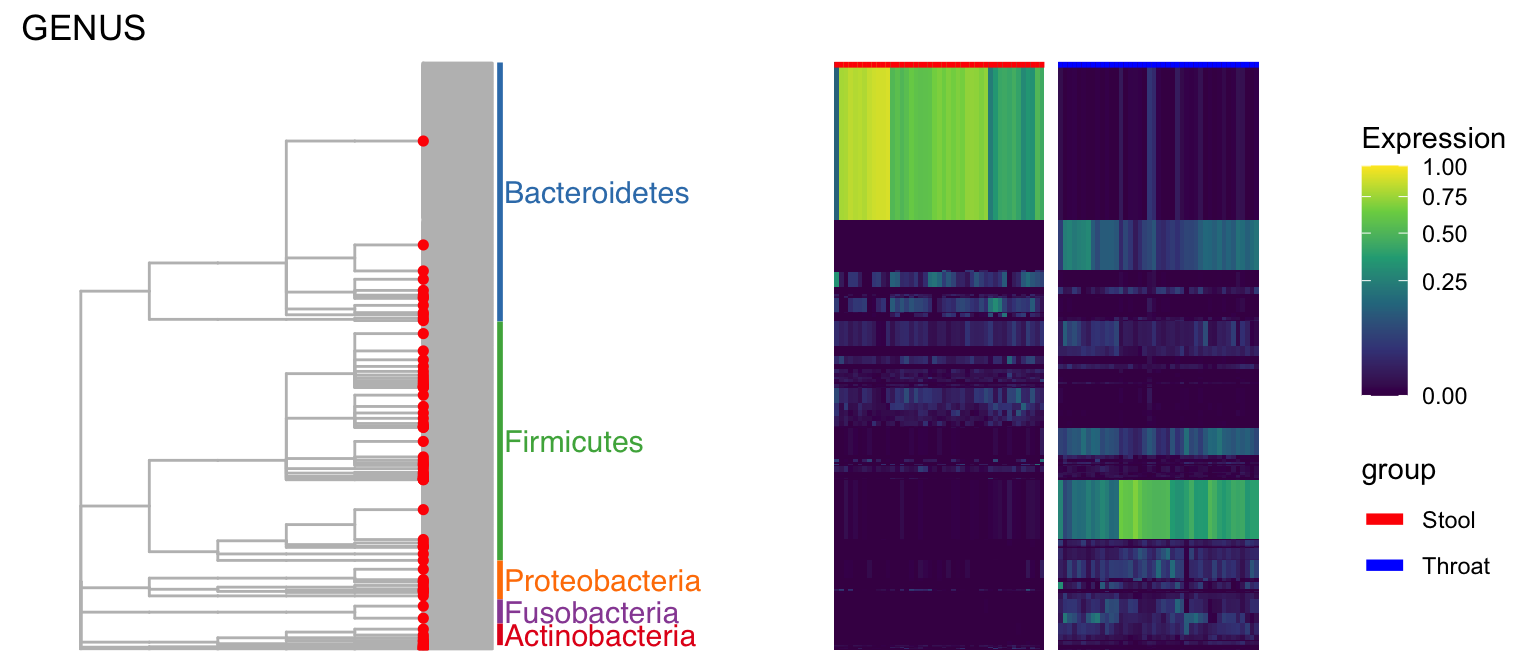
\includegraphics{figure/unnamed-chunk-69-1} \end{adjustwidth}

The heatmap at the geneus level of the tree could be generated in the same way. To avoid the repetition, we wrap the codes as a function \texttt{plotAssay} shown after the Figure \ref{fig:treehm}. Users could use it as a template or example to customize visualization function for the class \texttt{TreeSummarizedExperiment}.

\begin{Shaded}
\begin{Highlighting}[]
\NormalTok{sel_genus <-}\StringTok{ }\KeywordTok{c}\NormalTok{(}\StringTok{"GENUS:Bacteroides_1"}\NormalTok{, }\StringTok{"GENUS:Prevotella"}\NormalTok{,}
               \StringTok{"GENUS:Parabacteroides"}\NormalTok{, }\StringTok{"GENUS:Veillonella"}\NormalTok{,}
               \StringTok{"GENUS:Porphyromonas"}\NormalTok{, }\StringTok{"GENUS:Alistipes"}\NormalTok{)}
\NormalTok{fig2 <-}\StringTok{ }\KeywordTok{plotAssay}\NormalTok{(}\DataTypeTok{x =}\NormalTok{ agg_BCM, }
                  \DataTypeTok{taxo_level =} \StringTok{"GENUS"}\NormalTok{,}
                  \DataTypeTok{assay =} \DecValTok{2}\NormalTok{, }
                  \DataTypeTok{split_by =} \StringTok{"HMP_BODY_SUBSITE"}\NormalTok{, }
                  \DataTypeTok{clade_label =}\NormalTok{ sel_genus,}
                  \DataTypeTok{clade_fontsize =} \DecValTok{3}\NormalTok{,}
                  \DataTypeTok{clade_color =} \KeywordTok{brewer_pal}\NormalTok{(}\DataTypeTok{palette =} \StringTok{"Dark2"}\NormalTok{)(}\DecValTok{6}\NormalTok{),}
                  \DataTypeTok{gap_tree_heatmp =} \FloatTok{3.5}\NormalTok{,}
                  \DataTypeTok{rel_width =} \FloatTok{0.8}\NormalTok{, }
                  \DataTypeTok{anno_gap =} \DecValTok{50}\NormalTok{,}
                  \DataTypeTok{anno_color =} \KeywordTok{c}\NormalTok{(}\StringTok{"red"}\NormalTok{, }\StringTok{"navy"}\NormalTok{))}
\NormalTok{fig2}
\end{Highlighting}
\end{Shaded}

\begin{adjustwidth}{\fltoffset}{0mm}
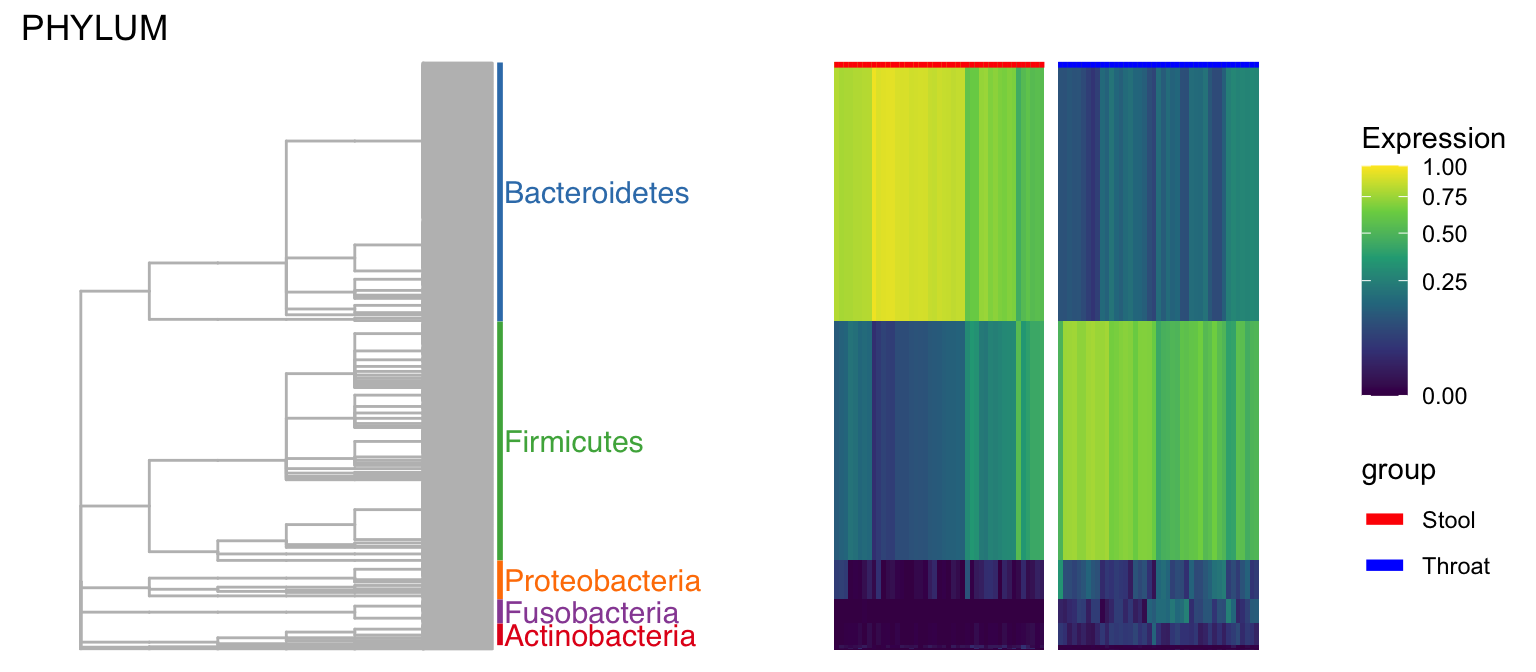
\includegraphics{figure/treehm-1} \end{adjustwidth}

\begin{Shaded}
\begin{Highlighting}[]
\NormalTok{plotAssay <-}\StringTok{ }\ControlFlowTok{function}\NormalTok{(x, }
                      \DataTypeTok{taxo_level =} \StringTok{"PHYLUM"}\NormalTok{, }\DataTypeTok{assay =} \DecValTok{1}\NormalTok{, }
                      \DataTypeTok{tree_fig =} \OtherTok{NULL}\NormalTok{, }\DataTypeTok{color_by =} \OtherTok{NULL}\NormalTok{, }
                      \DataTypeTok{split_by =} \OtherTok{NULL}\NormalTok{, }
                      \DataTypeTok{anno_gap =} \DecValTok{10}\NormalTok{, }\DataTypeTok{anno_color =} \OtherTok{NULL}\NormalTok{,}
                      \DataTypeTok{clade_label =} \OtherTok{NULL}\NormalTok{, }
                      \DataTypeTok{clade_fontsize =} \DecValTok{4}\NormalTok{,}
                      \DataTypeTok{clade_color =} \OtherTok{NULL}\NormalTok{,}
                      \DataTypeTok{gap_tree_heatmp =} \DecValTok{1}\NormalTok{, }\DataTypeTok{rel_width =} \DecValTok{1}\NormalTok{) \{}
  
  \CommentTok{# Tree}
\NormalTok{  rTree <-}\StringTok{ }\KeywordTok{rowTree}\NormalTok{(x)}
\NormalTok{  lab <-}\StringTok{ }\KeywordTok{c}\NormalTok{(rTree}\OperatorTok{$}\NormalTok{tip.label, rTree}\OperatorTok{$}\NormalTok{node.label)}
  
  \CommentTok{# level}
\NormalTok{  isLev <-}\StringTok{ }\KeywordTok{startsWith}\NormalTok{(lab, taxo_level)}
  \ControlFlowTok{if}\NormalTok{ (}\OperatorTok{!}\KeywordTok{sum}\NormalTok{(isLev)) \{}
    \KeywordTok{stop}\NormalTok{(}\StringTok{"Can't find nodes corresponding to the "}\NormalTok{, taxo_level, }\StringTok{" level."}\NormalTok{)}
\NormalTok{  \}}
\NormalTok{  lev <-}\StringTok{ }\NormalTok{lab[isLev]}
 
  \CommentTok{# assays}
\NormalTok{  sx <-}\StringTok{ }\KeywordTok{subsetByNode}\NormalTok{(}\DataTypeTok{x =}\NormalTok{ x, }\DataTypeTok{rowNode =}\NormalTok{ lev)}
  \ControlFlowTok{if}\NormalTok{ (}\KeywordTok{any}\NormalTok{(}\OperatorTok{!}\KeywordTok{dim}\NormalTok{(sx))) \{}
    \KeywordTok{stop}\NormalTok{(}\StringTok{"No data is available for plot"}\NormalTok{)}
\NormalTok{  \}}
\NormalTok{  cx <-}\StringTok{ }\KeywordTok{assays}\NormalTok{(sx)[[assay]]}
\NormalTok{  df_x <-}\StringTok{ }\KeywordTok{data.frame}\NormalTok{(cx, }\DataTypeTok{check.names =} \OtherTok{FALSE}\NormalTok{)}
  
  \CommentTok{# Tree figure}
  \ControlFlowTok{if}\NormalTok{ (}\KeywordTok{is.null}\NormalTok{(tree_fig)) \{}
\NormalTok{    tree_fig <-}\StringTok{ }\KeywordTok{ggtree}\NormalTok{(rTree, }\DataTypeTok{branch.length =} \StringTok{"none"}\NormalTok{, }\DataTypeTok{color =} \StringTok{"grey"}\NormalTok{) }\OperatorTok{+}
\StringTok{      }\KeywordTok{geom_point2}\NormalTok{(}\KeywordTok{aes}\NormalTok{(}\DataTypeTok{subset =}\NormalTok{ (label }\OperatorTok\StringTok{ }\NormalTok{lev)), }\DataTypeTok{color =} \StringTok{"red"}\NormalTok{,}
                  \DataTypeTok{size =} \FloatTok{1.2}\NormalTok{) }
\NormalTok{  \}}
  \ControlFlowTok{if}\NormalTok{ (}\OperatorTok{!}\KeywordTok{is.null}\NormalTok{(clade_label)) \{}
\NormalTok{     clade_node <-}\StringTok{ }\KeywordTok{transNode}\NormalTok{(}\DataTypeTok{tree =}\NormalTok{ rTree, }\DataTypeTok{node =}\NormalTok{ clade_label)}
     \ControlFlowTok{if}\NormalTok{ (}\KeywordTok{is.null}\NormalTok{(clade_color)) \{}
\NormalTok{       clade_color <-}\StringTok{ }\KeywordTok{rep}\NormalTok{(}\StringTok{"black"}\NormalTok{, }\KeywordTok{length}\NormalTok{(clade_label))}
\NormalTok{     \}}
     \ControlFlowTok{if}\NormalTok{ (}\KeywordTok{length}\NormalTok{(clade_color) }\OperatorTok{!=}\StringTok{ }\KeywordTok{length}\NormalTok{(clade_color)) \{}
       \KeywordTok{warning}\NormalTok{(}\StringTok{"clade_color has different lengths to clade_node."}\NormalTok{)}
\NormalTok{     \}}
\NormalTok{     clade_label <-}\StringTok{ }\KeywordTok{gsub}\NormalTok{(}\DataTypeTok{pattern =} \StringTok{".*:"}\NormalTok{, }\StringTok{""}\NormalTok{, clade_label)}
     \ControlFlowTok{for}\NormalTok{ (i }\ControlFlowTok{in} \KeywordTok{seq_along}\NormalTok{(clade_node)) \{}
\NormalTok{       tree_fig <-}\StringTok{ }\NormalTok{tree_fig }\OperatorTok{+}
\StringTok{         }\KeywordTok{geom_cladelabel}\NormalTok{(}\DataTypeTok{node  =}\NormalTok{ clade_node[i], }\DataTypeTok{label =}\NormalTok{ clade_label[i],}
                         \DataTypeTok{fontsize =}\NormalTok{ clade_fontsize, }\DataTypeTok{color =}\NormalTok{ clade_color[i])}
\NormalTok{     \}}
\NormalTok{  \}}
  \CommentTok{# split by}
\NormalTok{  colD <-}\StringTok{ }\KeywordTok{colData}\NormalTok{(sx)}
  \ControlFlowTok{if}\NormalTok{ (}\OperatorTok{!}\KeywordTok{is.null}\NormalTok{(split_by)) \{}
\NormalTok{    split_v <-}\StringTok{ }\NormalTok{colD[[split_by]]}
    \KeywordTok{names}\NormalTok{(split_v) <-}\StringTok{ }\KeywordTok{colnames}\NormalTok{(x)}
\NormalTok{  \} }\ControlFlowTok{else}\NormalTok{ \{}
\NormalTok{    split_v <-}\StringTok{ }\OtherTok{NULL}
\NormalTok{  \}}
  
  \CommentTok{# column annotation}
  \ControlFlowTok{if}\NormalTok{ (}\OperatorTok{!}\KeywordTok{is.null}\NormalTok{(anno_color)) \{}
\NormalTok{    un <-}\StringTok{ }\KeywordTok{unique}\NormalTok{(colD[[split_by]])}
    \ControlFlowTok{if}\NormalTok{ (}\KeywordTok{length}\NormalTok{(anno_color) }\OperatorTok{!=}\StringTok{ }\KeywordTok{length}\NormalTok{(un)) \{}
      \KeywordTok{stop}\NormalTok{(}\StringTok{"anno_color has length: "}\NormalTok{, }\KeywordTok{length}\NormalTok{(anno_color), }\StringTok{"; "}\NormalTok{, }
           \KeywordTok{length}\NormalTok{(un) , }\StringTok{" colors are expected"}\NormalTok{)}
\NormalTok{    \}}
    \KeywordTok{names}\NormalTok{(anno_color) <-}\StringTok{ }\NormalTok{un}
\NormalTok{  \}}
  \CommentTok{# column annotation}
\NormalTok{  f_heat <-}\StringTok{ }\KeywordTok{TreeHeatmap}\NormalTok{(}\DataTypeTok{hm_data =}\NormalTok{ df_x, }
                        \DataTypeTok{tree =}\NormalTok{ rTree, }
                        \DataTypeTok{tree_hm_gap =}\NormalTok{ gap_tree_heatmp,}
                        \DataTypeTok{tree_fig =}\NormalTok{ tree_fig,}
                        \DataTypeTok{column_split =}\NormalTok{ split_v,}
                        \DataTypeTok{column_split_gap =} \FloatTok{0.2}\NormalTok{, }
                        \DataTypeTok{column_anno =}\NormalTok{ split_v,}
                        \DataTypeTok{column_anno_gap =}\NormalTok{ anno_gap,}
                        \DataTypeTok{column_anno_size =} \DecValTok{4}\NormalTok{, }
                        \DataTypeTok{column_anno_color =}\NormalTok{ anno_color,}
                        \DataTypeTok{rel_width =}\NormalTok{ rel_width, }
                        \DataTypeTok{cluster_column =} \OtherTok{TRUE}\NormalTok{,}
                        \DataTypeTok{colnames_angle =} \DecValTok{45}\NormalTok{) }
\NormalTok{  f_heat}
  
\NormalTok{\}}
\end{Highlighting}
\end{Shaded}

\hypertarget{summary}{%
\section{Summary }\label{summary}}

This section is required if the paper does not include novel data or analyses. It allows authors to briefly summarize the key points from the article.

\hypertarget{software-availability}{%
\section{Software availability}\label{software-availability}}

The TreeSummarizedExperiment package is available at \url{https://www.bioconductor.org/packages/release/bioc/html/TreeSummarizedExperiment.html}

Source code of the development version of the package is available at \url{https://github.com/fionarhuang/TreeSummarizedExperiment}

\hypertarget{author-information}{%
\section{Author information}\label{author-information}}

Ruizhu Huang
Roles: Conceptualization, Software, Writing -- Original Draft Preparation, Writing -- Review \& Editing

Charlotte Soneson
Roles: Conceptualization, Supervision, Writing -- Review \& Editing

Mark D Robinson
Roles: Conceptualization, Supervision, Writing -- Review \& Editing

\hypertarget{competing-interests}{%
\section{Competing interests}\label{competing-interests}}

No competing interests were disclosed.

\hypertarget{grant-information}{%
\section{Grant information}\label{grant-information}}

Please state who funded the work discussed in this article, whether it is your employer, a grant funder etc. Please do not list funding that you have that is not relevant to this specific piece of research. For each funder, please state the funder's name, the grant number where applicable, and the individual to whom the grant was assigned. If your work was not funded by any grants, please include the line: `The author(s) declared that no grants were involved in supporting this work.'

\hypertarget{acknowledgments}{%
\section{Acknowledgments}\label{acknowledgments}}

We thank Héctor Corrada Bravo, Levi Waldron, Hervé Pagès, Martin Morgan, Ernst Felix G.M., Federico Marini, Jayaram Kancherla, Domenick Braccia, Guangchuang YU, Vince Carey, Kasper D Hansen, Kévin Rue-Albrecht, Davide Risso, Stephanie Hicks, Daniel van Twisk, Marcel Ramos and other members of the Bioconductor community for their helpful suggestions.

\hypertarget{refs}{}
\leavevmode\hypertarget{ref-R-SingleCellExperiment}{}%
Lun, Aaron, and Davide Risso. 2020. \emph{SingleCellExperiment: S4 Classes for Single Cell Data}.

\leavevmode\hypertarget{ref-R-SummarizedExperiment}{}%
Morgan, Martin, Valerie Obenchain, Jim Hester, and Hervé Pagès. 2020. \emph{SummarizedExperiment: SummarizedExperiment container}.

\leavevmode\hypertarget{ref-ape2019}{}%
Paradis, E, and K Schliep. 2019. ``ape 5.0: an environment for modern phylogenetics and evolutionary analyses in \{R\}.'' \emph{Bioinformatics} 35: 526--28.

\leavevmode\hypertarget{ref-Wang2019}{}%
Wang, Li-Gen, Tommy Tsan-Yuk Lam, Shuangbin Xu, Zehan Dai, Lang Zhou, Tingze Feng, Pingfan Guo, et al. 2019. ``Treeio: An R Package for Phylogenetic Tree Input and Output with Richly Annotated and Associated Data.'' \emph{Molecular Biology and Evolution} 37 (2): 599--603. \url{https://doi.org/10.1093/molbev/msz240}.

\leavevmode\hypertarget{ref-R-ggplot2}{}%
Wickham, Hadley, Winston Chang, Lionel Henry, Thomas Lin Pedersen, Kohske Takahashi, Claus Wilke, Kara Woo, Hiroaki Yutani, and Dewey Dunnington. 2020. \emph{ggplot2: Create Elegant Data Visualisations Using the Grammar of Graphics}. \url{https://cran.r-project.org/package=ggplot2}.

\leavevmode\hypertarget{ref-Yu2017}{}%
Yu, Guangchuang, David K. Smith, Huachen Zhu, Yi Guan, and Tommy Tsan Yuk Lam. 2017. ``Ggtree: An R Package for Visualization and Annotation of Phylogenetic Trees with Their Covariates and Other Associated Data.'' \emph{Methods in Ecology and Evolution} 8 (1): 28--36. \url{https://doi.org/10.1111/2041-210X.12628}.


\end{document}
